 	 \documentclass[aspectratio=169,handout]{beamer} %  [handout]  -> streicht die pause raus


\usepackage{dsfont} %Double stroke, e.g. for indicator function

%%%BASICS
\usepackage[utf8]{inputenc}
\usepackage{csquotes}
\usepackage{amssymb}

%%%START THEME SETTINGS

% IFO BLAU!!!
\setbeamercolor{structure}{fg=beamer@ifoblue}
\definecolor{beamer@ifoblue}{RGB}{12,50,82}
%\definecolor{ifoblue}{RGB}{12,50,82}

\usetheme{Hannover}
\usecolortheme{dolphin}
\usefonttheme{professionalfonts}

\usepackage{threeparttable} % add notes below tables
\renewcommand\TPTrlap{}		% add margins on the side of the notes
	\renewcommand\TPTnoteSettings{%
	\setlength\leftmargin{5 pt}%
	\setlength\rightmargin{5 pt}%
}

\usepackage{eurosym}

%path to tables
\makeatletter
\def\input@path{{../../analysis/tables/}}	%PATH TO TABLES
%or: \def\input@path{{/path/to/folder/}{/path/to/other/folder/}}
\usepackage[
center, format=plain,
font=normalsize,
nooneline,
labelfont={bf}
]{caption} 

%%%END THEME SETTINGS

\usepackage[compatibility=false]{caption}
\usepackage{subcaption}
\usepackage{graphicx} 
%PATH MAC
%\graphicspath{{/Users/marcfabel/Dropbox/Uni/Tinbergen/MPhil/STATA/GRAPHS/}}

%F:\_MPhil\STATA\graphs
%PATH Windows
%\graphicspath{{F:/_MPhil/STATA/graphs/}}
%\graphicspath{{C:/Users/fabel/Dropbox/Uni/Tinbergen/MPhil/STATA/GRAPHS/}}

\usepackage{afterpage}
 \usepackage{hyperref}
\usepackage{booktabs}
\usepackage[labelfont=bf,labelsep = period, singlelinecheck=off,justification=raggedright]{caption}%both together help to have subfigures, other specifications which are nice: labelformat = parens -> number in paranthesis
\usepackage[singlelinecheck=on]{subcaption}


\setbeamertemplate{items}[circle]
\usepackage{tikz}
\newcommand\mynum[1]{%
  \usebeamercolor{enumerate item}%
  \tikzset{beameritem/.style={circle,inner sep=0,minimum size=2ex,text=enumerate item.bg,fill=enumerate item.fg,font=\footnotesize}}%
  \tikz[baseline=(n.base)]\node(n)[beameritem]{#1};%
}	% the three packages are used to have enumerate points in text



%\usepackage{footmisc}

%\renewcommand{\thefootnote}{\fnsymbol{footnote}}
\let\vec\mathbf				 % make vector bold, with no arrow and not in italic


\title[Maternity leave and long-run child health]{  \textbf{Maternity Leave and Long-term Health Outcomes of Children}\newline Work in progress}
%\author[Danzer \& Fabel]{Natalia Danzer \& Marc Fabel \newline University of Munich \& ifo Institute}
\author[Danzer \& Fabel]{Natalia Danzer{\small \inst{1}} \and Marc Fabel {\small \inst{2}}}
\institute[]{\inst{1} Free University of Berlin, IZA, CESifo
	\and \vspace{-0.5em}
    \inst{2} Munich Graduate School of Economics \& ifo Institute at the University of Munich}
%\institute[VfS Meeting 2017]{}
\vspace{-2 em}
\date{American Economic Association meeting, Atlanta\\January 04, 2019}

\titlegraphic{
%\vspace{0.5em}

\vspace*{\fill} ~%

\includegraphics[height=0.8cm]{mgse_logo.jpg}
\hspace*{\fill}
   
\includegraphics[height=0.8cm]{logo_ifo.eps}

}

 \setbeamercovered{dynamic}				% macht die Pausen transparent

\captionsetup[figure]{labelformat=empty}
\captionsetup[table]{labelformat=empty}

%-=-=-=-=-=-=-=-=-=-=-=-=-=-=-=-=-=-=-=-=-=-=-=-=
%	NOTES:
%-=-=-=-=-=-=-=-=-=-=-=-=-=-=-=-=-=-=-=-=-=-=-=-=

%\AtBeginSection[]
%  {
%     \begin{frame}<beamer>
%     \frametitle{Agenda}
%     \tableofcontents[currentsection]
%     \end{frame}
%  }
% COMMAND UM ÜBERALL DIE ÜBERSICHT ZU HABEN

% To Do:
% overview slide?
% Channels, maternal employment (gibt zwei richtungen, siehe Natalia Email)



\begin{document}

\begin{frame}
	\titlepage
\end{frame}



%-=-=-=-=-=-=-=-=-=-=-=-=-=-=-=-=-=-=-=-=-=-=-=-=
%	INTRODUCTION:
%-=-=-=-=-=-=-=-=-=-=-=-=-=-=-=-=-=-=-=-=-=-=-=-=
%------------------------------------------------------
\section{Introduction}
\begin{frame}{Motivation}
\begin{block}{Early childhood conditions}
\begin{itemize}
\item great impact on later life outcomes (Almond \& Currie 2011, ...) 
\item multidimensional: health shocks (infections), toxic exposure (radiation), home environment (maternal employment), ...\pause
\item scope for public policy: \textbf{maternity leave mandates} - originally established with the goal to protect against job dismissal and damages to maternal and infant health, and secure standards of living by compensating income losses; allow to take a break from work and focus on child care\pause
\item effects of leave schemes have been examined a lot $\rightarrow$ add one piece to the puzzle \pause
\end{itemize}
\end{block}

\vspace{-0.5em}
\begin{block}{Research question}
\textbf{$\Rightarrow$ What are the causal effects of the length of maternity leave on children's health in the long-run?}
\end{block}

\end{frame}



% % TANYA WILSON has a quick overview: 
% \begin{frame}{This paper}
% \textbf{intervention}
% 1979 reform, in which ML was increased from blub to bla

% \textbf{outcome}
% hospital admission and special diagnoses chapters (ICD-code)

% \textbf{data}
% large admin data with high-quality measurements

% \textbf{identification}
% DiD
% \end{frame}
% % and maybe preview of results
% % and include maybe a historic picture (coverpage of Bundesgesetzblatt- abgespeichert in Bildern presentations)



%------------------------------------------------------
\begin{frame}{\mbox{Evaluation: 1979 Reform in West Germany}}



%\bigskip\bigskip
%\only<2>{
\begin{columns}
	\begin{column}{.6\textwidth}
		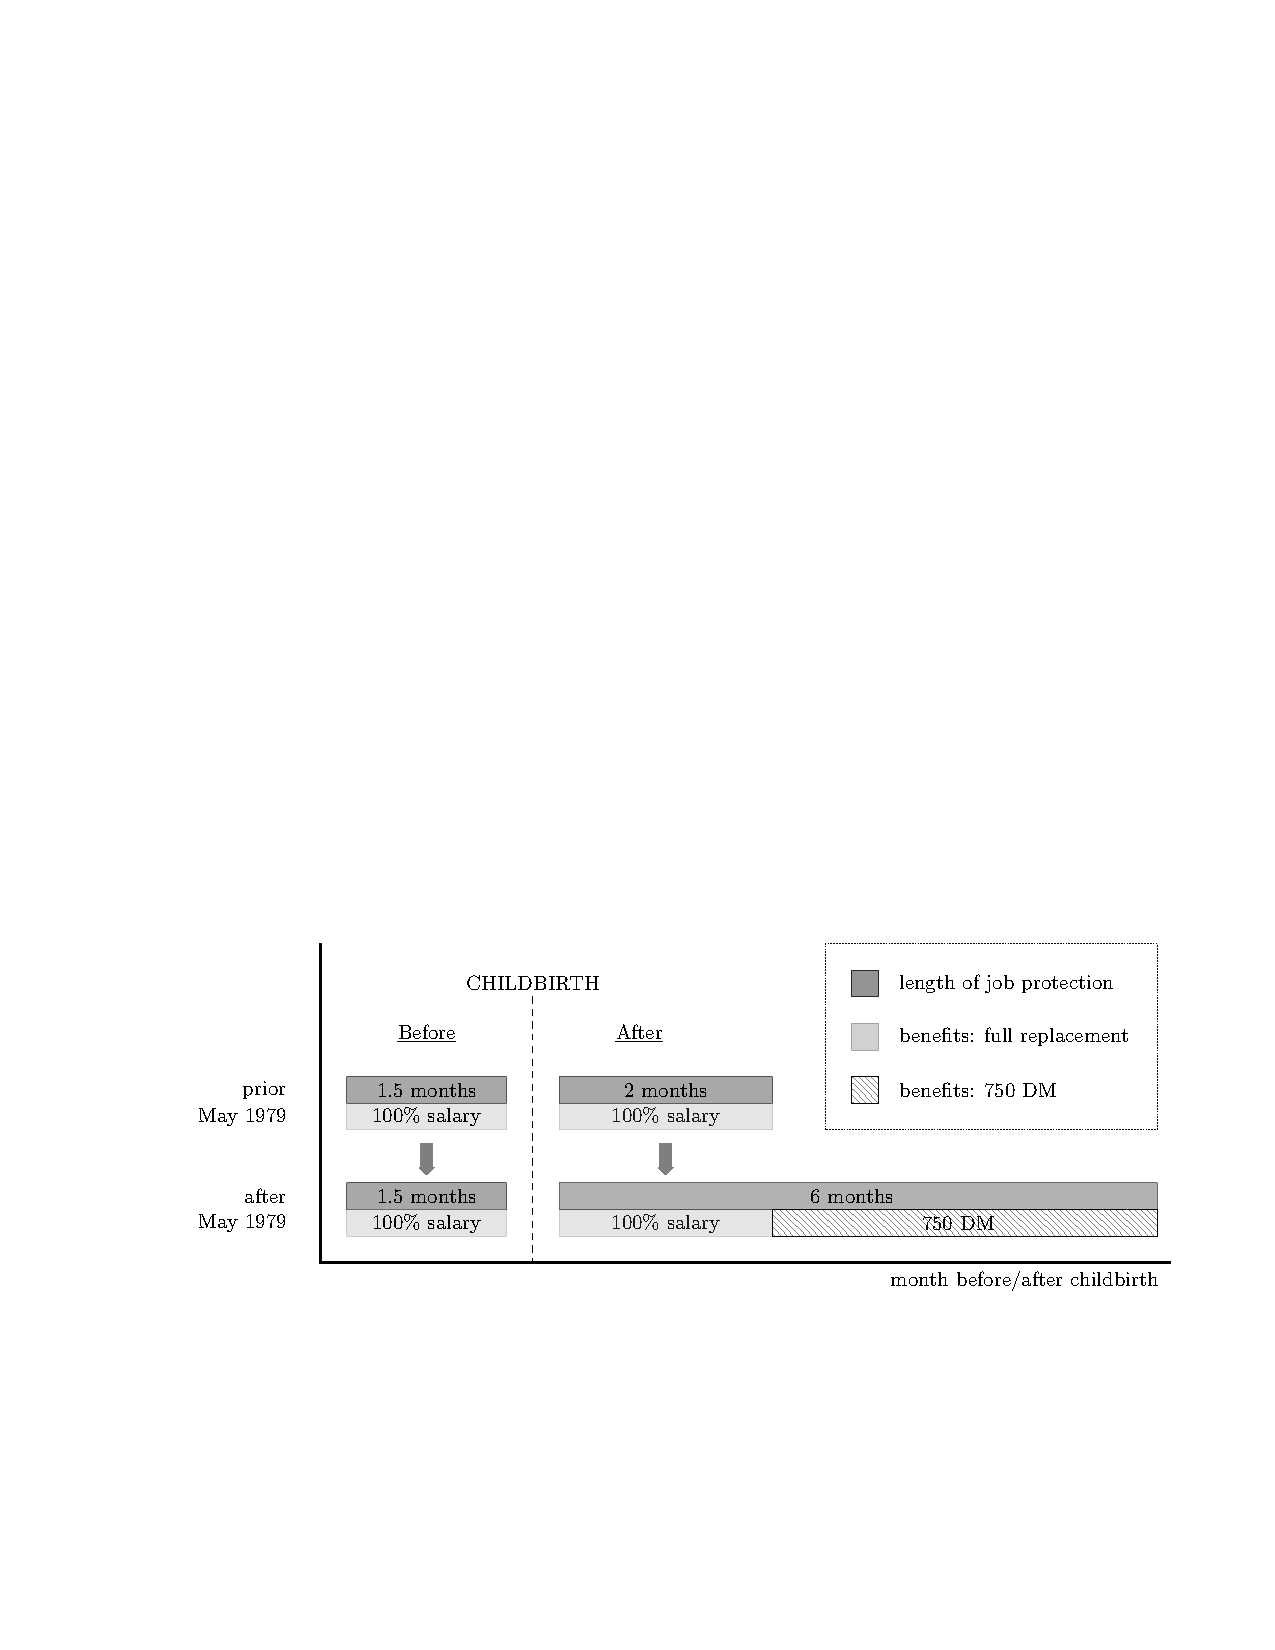
\includegraphics[width = \textwidth]{../../analysis/graphs/presentation/reform.pdf}
	\end{column}%
	\begin{column}{.40\textwidth}
		\textbf{Exogenous variation in maternity leave:}\begin{itemize}
		\item Extension in paid leave by four months
		\item Universal eligibility for working women
		\item Approx. take-up 40\%
		
		\end{itemize}
	\end{column}%
	\hfill
	
\normalsize
\end{columns}\pause
%}
\vspace{0.5 em}
\textbf{First stage:}
\begin{itemize}
\item Share of mothers who had returned to work by third month after childbirth is reduced by 30 pp ($\tfrac{2}{3}$ of reduction due to decline in full-time work)	
\item Labor supply is cut down, on average, by 0.835 months
\item Increase of cumulative available income by on average 1,700 DM (low wage mothers benefit more)
\end{itemize}
\end{frame}
		
%------------------------------------------------------
%general secion of channels
\begin{frame}{Channels: Length of ML $\rightarrow$ LR child health outcomes?}
	\begin{block}{Barker Hypothesis}\pause
		% \begin{itemize}
			% \item \textbf{Cumulative process (allostatic load)}
			% \begin{itemize}
			% 	\item stressful events are experienced repeatedly until chronic health impairments emerge eventually\pause
			% \end{itemize}
			\textbf{Biological embedding during sensitive periods}
			\begin{itemize}
				\item developing brain circuits are more receptive to environmental signals
				\item programming activity culminates in the first years of life (Räikkönen et al., 2012)
				\item infancy: hippocampus (regulation of emotions, social behavior, stress responsiveness, and ultimately mental health, Shonkoff et al., 2009)
				\item \emph{timing} and \emph{type} of experience matter\pause
			\end{itemize}
		% \end{enumerate}
		effects of experience may be \textbf{latent} at first, lag of many years (even decades) possible
	\end{block}	
\end{frame}
%------------------------------------------------------
% Channels: what was affected by the reform
\begin{frame}
\begin{block}{Potential changes in children's environment due to the reform}
\begin{enumerate}
\item \textbf{More maternal time during crucial time period for child development} {\mynum{+} }\vspace{-0.25 em}
\begin{itemize}
\item[-]Breastfeeding (Baker and Milligan, 2008)
\begin{itemize}
\item medical advantages (Horta et al., 2007)
\item stronger mother-child bond $\rightarrow$ crucial for cognitive development (Klaus, 1998); associated with less behavioral problems (Brooks-Gunn et al., 2002)
\end{itemize}
\item[-]Better monitor child's health status and more timely doctor visits (Berger et al., 2005)

\item[-] Prepare healthier meals and lower risk of injuries and infectious disease (Morrill, 2011)\pause
\end{itemize}

\item \textbf{Changes in parental health outcomes} {\mynum{+} }, e.g. stress, depression, poor health $\rightarrow$ affect ability to nurture (Beuchert et al., 2014; Crnic et al., 2005)\pause
\item \textbf{Changes in HH income} {\mynum{+} }
\begin{itemize}
\item association with educational attainment (Dahl and Lochner, 2012), child health (Hoynes et al., 2015) \& brain development (Duncan et al, ongoing)
%\item reduced income share $\rightarrow$ expenditure for child goods (Lundberg and Pollak, 1996)
\end{itemize}

% \item \textbf{Effects on higher-order fertility} \mynum{-} (Lalive and Zweimüller, 2009); quantity of children and birth spacing
\end{enumerate}
\end{block}
\end{frame}



%------------------------------------------------------
% \begin{frame}{Literature}
% \textbf{Previous Literature:}
% \begin{enumerate}
% \item \underline{Long-term effects of maternity leave}\\ Inconclusive and more emphasis on educational attainment and labor market outcomes
% \item \underline{Maternity leave $\rightarrow$ health (both maternal and infant)} \\only short-run effects
% \end{enumerate}\pause
% \bigskip
% $\Rightarrow$ \textbf{Contribution to the literature:}
% \begin{itemize}
% \item Adding to the scarce evidence on health outcomes, in particular in the long-run and mental health

% \item Causal ITT effects of maternity leave in the first year based on large administrative data sets

% \item life-course perspective: observing the children over a long time horizon (age 16-35)

% \end{itemize}
% \end{frame}
%------------------------------------------------------



%-=-=-=-=-=-=-=-=-=-=-=-=-=-=-=-=-=-=-=-=-=-=-=-=
%	IDENTIFICATION STRATGEY:
%-=-=-=-=-=-=-=-=-=-=-=-=-=-=-=-=-=-=-=-=-=-=-=-=
\section{Identification}
%------------------------------------------------------
\begin{frame}{Difference-in-Difference Regression Discontinuity}
\label{BACK_FROM_VALIDITY}
Estimation strategy following Dustmann and Schönberg (2012),...: eradicate season-of-birth effects
\begin{align*}
%\resizebox{.99 \textwidth}{!} {$
%Y_{imt} = \gamma_0 + \gamma_1 T_{im} + \gamma_2 After_{im}+ \color{red}\gamma_3 \color{black}T_{im} \times After_{im} + \vec{D}_{im}'\psi +\xi_{imt} \\
Y_{mt} = \gamma_0 + \gamma_1 T_{m} + \gamma_2 After_{m}+ \color{red}\gamma_3 \color{black}(T_{m} \times After_{m}) + \psi_{m}  + \rho_t +\xi_{mt} 
%$}%\label{eq:RD+DD}
\end{align*}
\vspace{-0.5cm}
\begin{itemize}
\begin{scriptsize}
\item[-] $Y_{mt}$: number of diagnoses per thousand individuals in respective month-of-birth cohort
\item[-] $T_{m}$: treatment dummy equals one if individual is born in the treatment year
\item[-] $After_{m}$: dummy whether individual is born in/after May
\item[-] $T_{m} \times After_{m}$: interaction equals one for group of interest (born between May-Oct 1979 in the widest specification)
\item[-] $\psi_m,\ \rho_t$ birth month and year (wave) fixed effects
\item[-] local estimation: 3-6 months to the left/right of reform cut-off date
\item[-] \texttt{control} cohort: birth cohort one year prior to the reform
\item[-] Identifying assumption: seasonal part is time-invariant
\item[-] Intention-to-treat effect

\end{scriptsize}
\end{itemize}
\hyperlink{VALIDITY}{\beamerbutton{$\triangleright$ Validity: fertility distribution \& covariate balance}}
\end{frame}

%------------------------------------------------------

%-=-=-=-=-=-=-=-=-=-=-=-=-=-=-=-=-=-=-=-=-=-=-=-=
%	 DATA & VARIABLES:
%-=-=-=-=-=-=-=-=-=-=-=-=-=-=-=-=-=-=-=-=-=-=-=-=
\section{Data}\label{DATA}
\begin{frame}{Data \& Variables}\label{VARIABLES}
\textbf{Hospital administrative data (1995-2014):} 
\begin{itemize}
\item[-] Universe of German in-patient cases ($\approx 18$ Mio/year). \newline Information about patient's main diagnosis, age, gender, place of residence, date of admission and discharge. \hyperlink{DESCRIPTIVES}{\beamerbutton{$\triangleright$ descriptives}}
\item[-] Outcomes: 
\begin{itemize}
\item hospitalization (all diagnoses)
\item specific chapters according to the ICD classification system\newline e.g. mental and behavioral disorders ("F" chapter ICD-10, 12-18\% of all diagnoses in 2014 - most frequent diagnosis for age group 15 to 35 years)
\end{itemize}




 \hyperlink{ICD10 CLASSIFICATION}{\beamerbutton{$\triangleright$ ICD coding}}
\hyperlink{5 MOST COMMON DIAGNOSES}{\beamerbutton{$\triangleright$ most common diagnosis types per age group}}

\item[-] define dependent variable as number of cases per 1,000 individuals in the region of West-Germany

\item[-] level of analysis: cohort$\times$month-of-birth$\times$year

% \begin{itemize}
% \item due to psychoactive substance use \footnote{Acute intoxication, harmful use, dependence syndrome, withdrawal state, ...}
% \item schizophrenia
% \item mood [affective] disorders
% \item neurotic, stress-related and somatoform disorders
% \item disorders of adult personality and behavior
% \end{itemize}
\end{itemize}
%  \textbf{II) German Micro Census (2005-2013):}
% \begin{itemize}
% \item[-] used for additional analyses; not shown today
% \end{itemize} 
 
\end{frame}
%------------------------------------------------------


%-=-=-=-=-=-=-=-=-=-=-=-=-=-=-=-=-=-=-=-=-=-=-=-=
%	 ANALYSIS
%-=-=-=-=-=-=-=-=-=-=-=-=-=-=-=-=-=-=-=-=-=-=-=-=
\section{Analysis}

\subsection{Hospitalization}
%hauptttabelle (hospital2)
\begin{frame}{(1) Hospital admission (all inpatients)}\label{HOSPITAL_TAB_TOTAL}
	\tiny
	\vspace*{\fill}
\begin{table}[H] \centering 
 \begin{threeparttable} \centering %\caption{ITT effects on \textbf{hospital admission (total)}}\label{tab: DD_hopsital2_total}
  {\def\sym#1{\ifmmode^{#1}\else\(^{#1}\)\fi} 
 	\begin{tabular}{l*{6}{c}}
 		\toprule 
 		%\multicolumn{5}{l}{Dependant variable: \textbf{Hospital admission (total)}}\\ \\ 
 		& \multicolumn{5}{c}{Estimation window} \\ 
 		\cmidrule(lr){2-6}
 		&\multicolumn{1}{c}{(1)}&\multicolumn{1}{c}{(2)}&\multicolumn{1}{c}{(3)}&\multicolumn{1}{c}{(4)}&\multicolumn{1}{c}{(5)}\\
 		&\multicolumn{1}{c}{6M}&\multicolumn{1}{c}{5M}&\multicolumn{1}{c}{4M}&\multicolumn{1}{c}{3M}&\multicolumn{1}{c}{Donut}\\
 		\midrule
 		\multicolumn{5}{l}{\emph{Panel A. Over entire length of the life-course}} \\
 		\hspace*{10pt}Overall&      -2.218         &      -2.181\sym{*}  &      -1.944\sym{**} &      -2.168\sym{**} &      -2.713\sym{***}\\
                    &     (1.401)         &     (1.143)         &     (0.917)         &     (0.782)         &     (0.826)         \\
\midrule Dependent mean&       122.7         &       121.0         &       120.5         &       120.6         &       121.4         \\
Effect in SDs [\%]  &       19.22         &       18.84         &       17.35         &       19.78         &       24.62         \\
Observations        &         240         &         320         &         400         &         480         &         400         \\
 \\ \\
 		\multicolumn{5}{l}{\emph{Panel B. Age brackets}} \\
 		\hspace*{10pt}Age 17-21&      -1.095         &      -0.735         &      -0.590         &      -1.517\sym{+}  &      -1.963\sym{**} \\
                    &     (1.603)         &     (1.198)         &     (0.995)         &     (0.946)         &     (0.931)         \\
 \hspace*{10pt}Age 22-26&      -0.735         &      -0.667         &      -0.613         &      -0.611         &      -1.080         \\
                    &     (1.672)         &     (1.412)         &     (1.113)         &     (0.937)         &     (1.012)         \\
 \hspace*{10pt}Age 27-31&      -2.546\sym{*}  &      -3.209\sym{**} &      -3.015\sym{***}&      -2.665\sym{***}&      -2.974\sym{***}\\
                    &     (1.375)         &     (1.132)         &     (0.909)         &     (0.826)         &     (0.949)         \\
 \hspace*{10pt}Age 32-35&      -3.869\sym{***}&      -3.619\sym{**} &      -4.572\sym{***}&      -5.045\sym{**} &      -4.717\sym{***}\\
                    &     (1.083)         &     (1.277)         &     (1.460)         &     (1.721)         &     (1.191)         \\
 
 		\bottomrule 
 	\end{tabular}}
 	\begin{tablenotes} 
 		\item \tiny \emph{Notes:} Clustered standard errors are reported in parentheses. \newline Significance levels: $+$ p $<$ 0.15, * p $<$ 0.10, ** p $<$ 0.05, *** p $<$ 0.01. 
 	\end{tablenotes} 
 \end{threeparttable} 
 \end{table}
\vspace*{\fill}\clearpage 
	\hyperlink{HOSPITAL_TAB_WOMEN}{\beamerbutton{$\triangleright$ by gender}}
\end{frame}

 

%------------------------------------------------------
\subsection{Life-cycle}
\begin{frame}{(1) Hospitalization: life-cycle perspective}
\vspace{1 em}
\vspace{-0.7 em}
\begin{figure}\centering
\begin{subfigure}[h]{0.49\linewidth}\centering\caption{Women}
	\includegraphics[width=\linewidth]{../../analysis/graphs/presentation/lc_hospital2_female_gdr.pdf}
\end{subfigure}
\begin{subfigure}[h]{0.49\linewidth}\centering\caption{Men}
	\includegraphics[width=\linewidth]{../../analysis/graphs/presentation/lc_hospital2_male_gdr.pdf}
\end{subfigure}
\end{figure}
\end{frame}
%------------------------------------------------------
\subsection{Chapters}\label{CHAPTERS_TOTAL}
\begin{frame}{(2) Effect distribution across diagnosis chapters}
	\begin{figure}\centering
		\includegraphics[width=0.7\linewidth]{../../analysis/graphs/presentation/effect_chapters_frequency.pdf}
	\end{figure}
	\hyperlink{CHAPTERS_FEMALE}{\beamerbutton{$\triangleright$ by gender}}
\end{frame}


\begin{frame}{Summary}
Effects on hospital admission...
	\begin{itemize}	
		\item results are driven by men
		\item differentials are opening up from the age of 28 onwards
		\item largest effect stemming from mental \& behavioral disorders (absolute and relative (\% of baseline mean))
	\end{itemize}	
\end{frame}



%------------------------------------------------------
\subsection{Mental disorders}\label{MBD_TAB_TOTAL}
\begin{frame}{(3) Mental \& behavioral disorders (all in-patients)}\tiny
	\vspace*{\fill}
\begin{table}[H] \centering 
 \begin{threeparttable} \centering %\caption{ITT effects on \textbf{mental \& behavioral disorders (total)}}\label{tab: DD_d5_total}
  {\def\sym#1{\ifmmode^{#1}\else\(^{#1}\)\fi} 
 	\begin{tabular}{l*{6}{c}}
 		\toprule 
 		%\multicolumn{5}{l}{Dependant variable: \textbf{Hospital admission (total)}}\\ \\ 
 		& \multicolumn{5}{c}{Estimation window} \\ 
 		\cmidrule(lr){2-6}
 		&\multicolumn{1}{c}{(1)}&\multicolumn{1}{c}{(2)}&\multicolumn{1}{c}{(3)}&\multicolumn{1}{c}{(4)}&\multicolumn{1}{c}{(5)}\\
 		&\multicolumn{1}{c}{6M}&\multicolumn{1}{c}{5M}&\multicolumn{1}{c}{4M}&\multicolumn{1}{c}{3M}&\multicolumn{1}{c}{Donut}\\
 		\midrule
 		\multicolumn{5}{l}{\emph{Panel A. Over entire length of the life-course}} \\
 		\hspace*{10pt}Overall&      -0.656         &      -0.852\sym{**} &      -0.756\sym{**} &      -0.634\sym{**} &      -0.809\sym{***}\\
                    &     (0.420)         &     (0.350)         &     (0.280)         &     (0.249)         &     (0.274)         \\
\midrule Dependent mean&       19.23         &       19.05         &       18.98         &       18.96         &       19.16         \\
Effect in SDs [\%]  &       11.33         &       14.87         &       13.36         &       11.43         &       14.64         \\
Observations        &         240         &         320         &         400         &         480         &         400         \\
 \\ \\
 		\multicolumn{5}{l}{\emph{Panel B. Age brackets}} \\
 		\hspace*{10pt}Age 17-21&       0.135         &       0.318         &       0.268         &       0.174         &     -0.0603         \\
                    &     (0.516)         &     (0.387)         &     (0.314)         &     (0.263)         &     (0.239)         \\
 \hspace*{10pt}Age 22-26&       0.343         &      -0.172         &      -0.146         &    -0.00769         &      -0.360         \\
                    &     (0.640)         &     (0.607)         &     (0.500)         &     (0.420)         &     (0.454)         \\
 \hspace*{10pt}Age 27-31&      -1.258\sym{**} &      -1.508\sym{***}&      -1.301\sym{***}&      -1.000\sym{**} &      -1.020\sym{**} \\
                    &     (0.546)         &     (0.478)         &     (0.391)         &     (0.357)         &     (0.433)         \\
 \hspace*{10pt}Age 32-35&      -1.886\sym{***}&      -2.352\sym{***}&      -1.906\sym{***}&      -1.949\sym{***}\\
                    &     (0.224)         &     (0.305)         &     (0.372)         &     (0.439)         \\
 
 		\bottomrule 
 	\end{tabular}}
 	\begin{tablenotes} 
 		\item \tiny \emph{Notes:} Clustered standard errors are reported in parentheses. \newline Significance levels: $+$ p $<$ 0.15, * p $<$ 0.10, ** p $<$ 0.05, *** p $<$ 0.01.
 	\end{tablenotes} 
 \end{threeparttable} 
 \end{table}
\vspace*{\fill}\clearpage 
	\hyperlink{MBD_TAB_WOMEN}{\beamerbutton{$\triangleright$ by gender}}
\end{frame}	





\subsection{Life-cycle}
\begin{frame}{(3) MBD: life-cycle perspective}
\vspace{1 em}
\vspace{-0.7 em}
\begin{figure}\centering
\begin{subfigure}[h]{0.49\linewidth}\centering\caption{Women}
	\includegraphics[width=\linewidth]{../../analysis/graphs/presentation/lc_d5_female_gdr.pdf}
\end{subfigure}
\begin{subfigure}[h]{0.49\linewidth}\centering\caption{Men}
	\includegraphics[width=\linewidth]{../../analysis/graphs/presentation/lc_d5_male_gdr.pdf}
\end{subfigure}
\end{figure}
\end{frame}


%------------------------------------------------------
\subsection{Subcategories}
\begin{frame}{(4) Results per subcategory}
\begin{figure}\centering
\begin{subfigure}[h]{0.49\linewidth}\centering\caption{ITT effects}
	\includegraphics[width=\linewidth]{../../analysis/graphs/presentation/effect_d5.pdf}
\end{subfigure}
\begin{subfigure}[h]{0.49\linewidth}\centering\caption{Diagnosis distribution over time}
	\includegraphics[width=\linewidth]{../../analysis/graphs/presentation/fig_d5_partition.pdf}
\end{subfigure}
\end{figure}
\end{frame}




%------------------------------------------------------
% ROBUSTNESS SECTION
\subsection{Robustness}

\begin{frame}{(5) Robustness}\label{ROBUSTNESS}
	The results are robust to: 
	\begin{itemize}
		\item Alternative \textbf{specifications}: 
		\begin{itemize}
			\item denominator: current population (approximated)
			\item level of analysis: labor-market region \hyperlink{MAP_LMR}{\beamerbutton{$\triangleright$ map}}
		\end{itemize}
		\item Alternative \textbf{estimation}:
		\begin{itemize}
			\item triple difference model
			\item DD with East Germany
			\item more control cohorts
		\end{itemize}
		\item \textbf{Placebos}: temporal and spatial
		\item \textbf{Heterogeneity}: effects are larger in urban areas
	\end{itemize}
	\vspace*{1em}
	\hyperlink{ROBUSTNESS_TABLE}{\beamerbutton{$\triangleright$ Table}}
	\hyperlink{RD_PLOTS}{\beamerbutton{$\triangleright$ RD plots}}
\end{frame}










%-=-=-=-=-=-=-=-=-=-=-=-=-=-=-=-=-=-=-=-=-=-=-=-=
%	 SUMMARY
%-=-=-=-=-=-=-=-=-=-=-=-=-=-=-=-=-=-=-=-=-=-=-=-=
\section{Conclusion}
\begin{frame}{Concluding remarks}
\begin{itemize}
%\item \textbf{Points of concern:}
%\begin{enumerate}
%\item Eligibility universal, but take-up not (40\%) $\rightarrow$ selection on unobservables?
%\item Coincidence with peak of second oil crisis, macroeconomic situation at time of conception matters (Dehejia and Lleras-Muney, 2004) $\rightarrow$ one cohort significantly different affected than the other?
%\end{enumerate}
\item \textbf{Summary:}\label{CONCLUSION}
\begin{itemize}
%\item {Large transfer payments involved:} German ministry of family affairs spent $6$ billion Euros in 2016 ($\sim2\%$ entire federal government budget)
\item A large body of the literature finds mixed effects on other outcomes (SES) - long-run health outcomes (in particular mental health) have not been in the center of the discussion

\item Our results suggest that ML reform had significantly positive effects on child mental health in the long run.

\item Goal of ML: improve welfare of mothers and children

\item some benefits of ML materialize later and in other dimensions than what policy makers had in mind originally:  saving of EUR 7.0 million in 2014 for MBD \newline  (720 fewer diagnoses $\times$ EUR 9,823)



 % 720 fewer diagnoses of MBD (from $\sim$ 300,000 individuals) in 2014, one diagnosis costs on average EUR 9,823 \newline $\Rightarrow$ saving 

\end{itemize}
\end{itemize}

\hyperlink{MZ}{\beamerbutton{$\triangleright$ further results Micro Census: health \& socio-economic outcomes}}


\end{frame}




%-=-=-=-=-=-=-=-=-=-=-=-=-=-=-=-=-=-=-=-=-=-=-=-=
%	 THANK YOU
%-=-=-=-=-=-=-=-=-=-=-=-=-=-=-=-=-=-=-=-=-=-=-=-=
\begin{frame}
\begin{center}
Thank you very much for your attention!\newline Email: \texttt{fabel@ifo.de}
\end{center}




\end{frame}

%\section*{Appendix}
%\begin{frame}
%Restlichen Abbildungen, backup slides
%\end{frame}


%-=-=-=-=-=-=-=-=-=-=-=-=-=-=-=-=-=-=-=-=-=-=-=-=
%	 APPENDIX
%-=-=-=-=-=-=-=-=-=-=-=-=-=-=-=-=-=-=-=-=-=-=-=-=
\section*{Appendix}
%------------------------------------------------------
\subsection*{Validity}
%------------------------------------------------------
\label{VALIDITY}
\begin{frame}{Validity}
Problem: Behavioral responses with respect to the running variable. Is birth a random variable $\sim$ $\mathcal{N}(40w,2w)$?
\begin{itemize}
\item \textbf{Strategic conception}\newline draft bill does not allow to react to reform (4 months before reform put into practice), media coverage (earliest 2 months)

\item \textbf{Postponing induced births and cesarean sections}\newline Gans \& Leigh (2009): Australian baby bonus\newline $\rightarrow$ similar distortionary ”introduction effects”?



\begin{enumerate}
\item Timing of birth $\rightarrow$ fertility distribution
\item Parental pre-determined covariate balance
\end{enumerate}
\end{itemize}
\medskip
$\Rightarrow$ No indication of sorting, occurrence of birth is a random event; policy change can be seen as true quasi-experiment \newline $\Rightarrow$ Additional robustness check: Donut specification

 \hyperlink{BACK_FROM_VALIDITY}{\beamerbutton{Back to identification}}

\end{frame}
%------------------------------------------------------
\begin{frame}{Validity I}
	\begin{figure}
		\includegraphics[width=0.69\textwidth]{../../analysis/graphs/presentation/fig_validity_births}
	\end{figure}
	\begin{center}\vspace{-1em}
		\tiny \flushleft Note:  The figure displays the daily number of birth, both raw and when accounting for day of year, public holiday, and year$\times$day of week fixed effects. Source: Destatis.
	\end{center}
	\hyperlink{BACK_FROM_VALIDITY}{\beamerbutton{Back to identification}}
\end{frame}
%------------------------------------------------------
% Regression results
\begin{frame}{Validity II: regression results}
	\begin{figure}
		\includegraphics[width=0.55\textwidth]{../../analysis/graphs/presentation/fig_validity_regression}
	\end{figure}
	
	\hyperlink{BACK_FROM_VALIDITY}{\beamerbutton{Back to identification}}
\end{frame}
%------------------------------------------------------
% ALL YEARS FERTILITY HISTOGRAM
\begin{frame}{Validity III: Fertility distribution}
\begin{figure}
\begin{tikzpicture}
	\node[anchor=south west,inner sep=0] at (0,0) {\includegraphics[width=0.99\textwidth]{../../analysis/graphs/presentation/fig_validity_histograms}};
	%\draw[red,ultra thick,rounded corners] (5.2,0) rectangle (10.3,4.3);
	\end{tikzpicture}
\end{figure}
\begin{center}\vspace{-1em}
\tiny \flushleft Note:  The figures display the relative frequency of birth months per birth cohort, adjusted for different lengths of the months.  Source: Destatis.
\end{center}\hyperlink{BACK_FROM_VALIDITY}{\beamerbutton{Back to identification}}
\end{frame}
%------------------------------------------------------
% PARENTAL COVARIATE BALANCE TABLE
\begin{frame}{Validity IV: Balancing table}
\begin{figure}
\textbf{Pre-determined covariate balance}
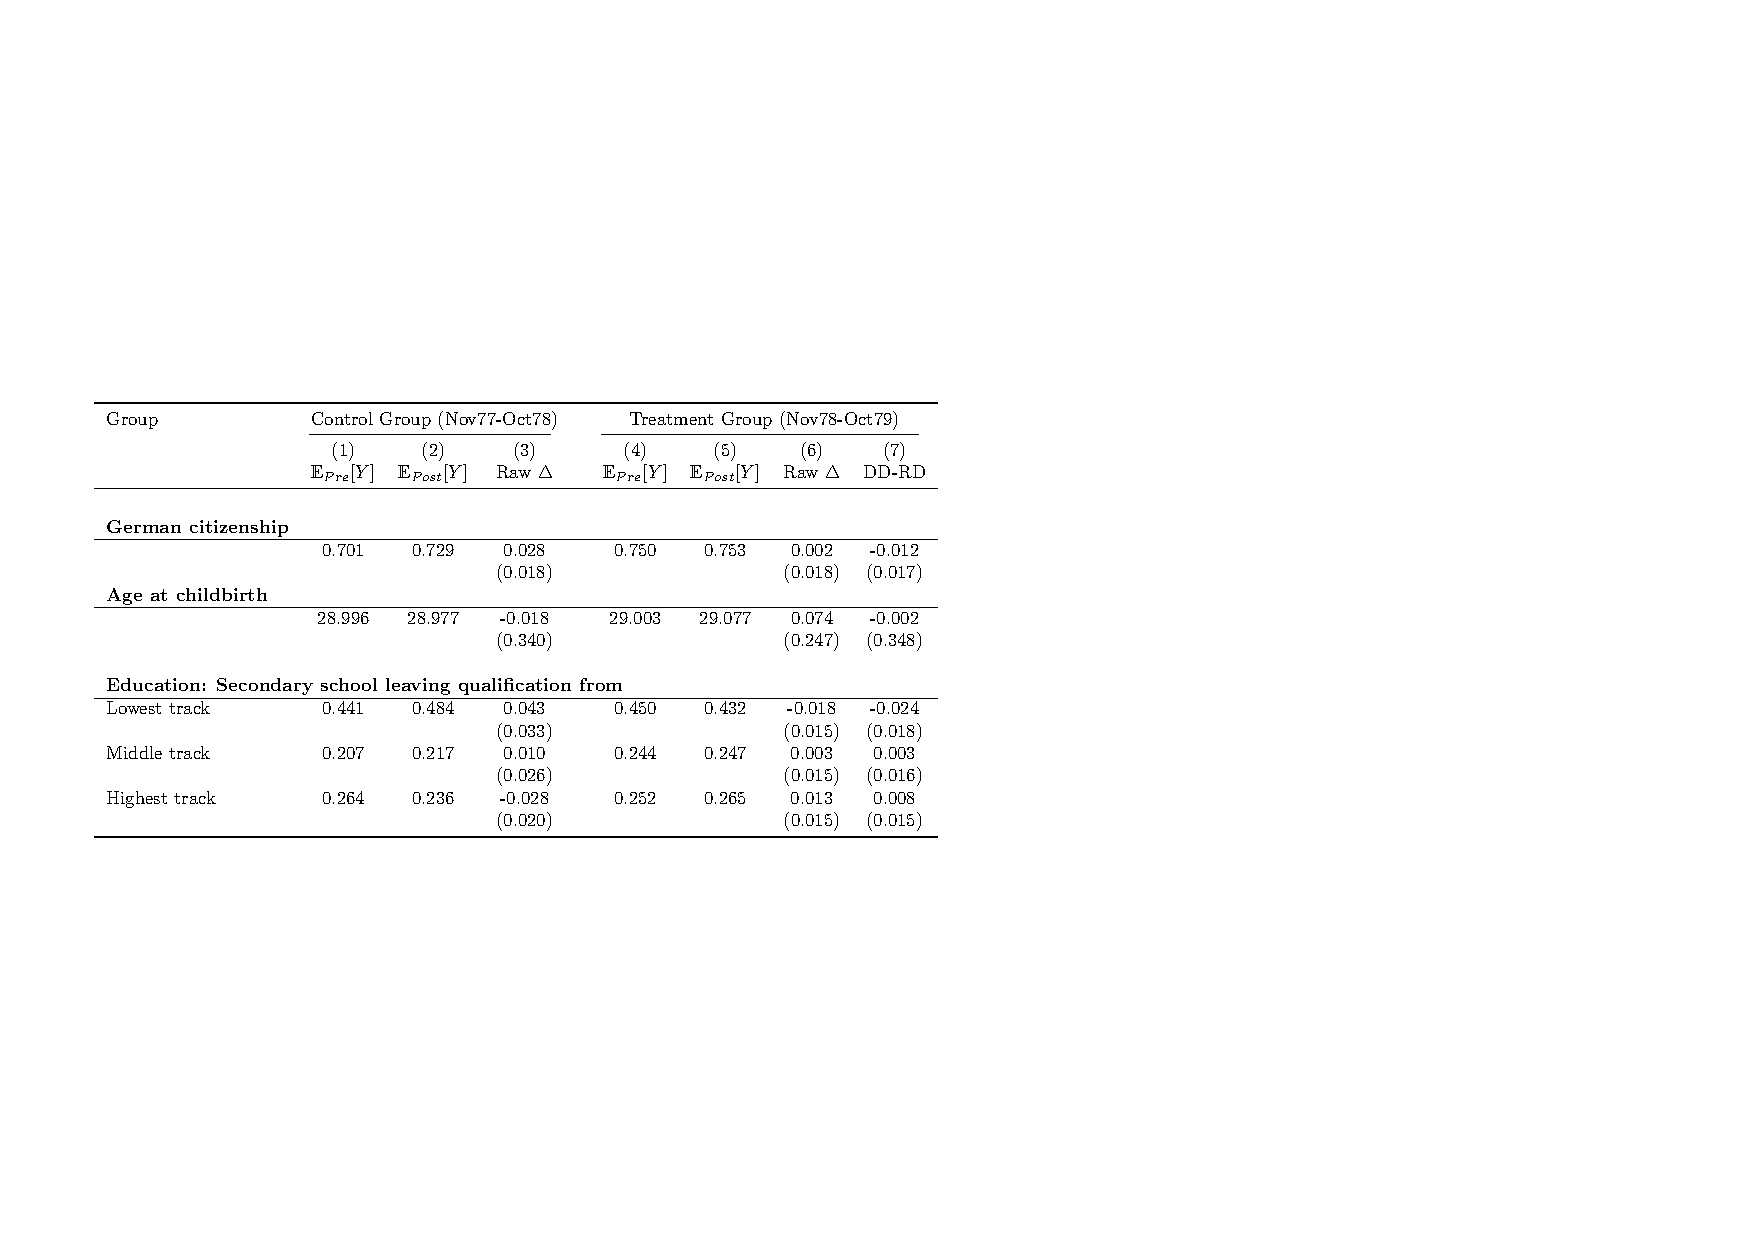
\includegraphics[width=0.8\linewidth]{../../analysis/graphs/presentation/parental_covariate_balance}
\end{figure}
\begin{minipage}{0.9\linewidth}
\begin{center}\vspace{-1cm}
\tiny \flushleft Note: The table compares parental characteristics within half a year around the threshold. It reports difference-in-means and DD-RD estimates. Source: German Micro Census, waves 2005, 2009 and 2013. 
\end{center}
\end{minipage}

\hyperlink{BACK_FROM_VALIDITY}{\beamerbutton{Back to identification}}
\end{frame}
%------------------------------------------------------

% DATA
\begin{frame}{Hospitalization}\label{DESCRIPTIVES}
	\begin{figure}
		\includegraphics[width=0.7\linewidth]{../../analysis/graphs/presentation/fig_hospital_admission.pdf}
	\end{figure}
	\hyperlink{DATA}{\beamerbutton{$\triangleright$ back}}
\end{frame}


%------------------------------------------------------
\begin{frame}{Outcome classification}
\label{ICD10 CLASSIFICATION}
\begin{figure}
	\includegraphics[width=0.85\linewidth]{../../analysis/graphs/presentation/tab_summary.pdf}
\end{figure}
\hyperlink{VARIABLES}{\beamerbutton{Back to data \& variables}}
\end{frame}

\begin{frame}{Outcome classification: MBD}
\begin{figure}
	\includegraphics[width=0.85\linewidth]{../../analysis/graphs/presentation/tab_summary_d5.pdf}
\end{figure}
\hyperlink{VARIABLES}{\beamerbutton{Back to data \& variables}}
\end{frame}


%------------------------------------------------------
% 5 most common diagnoses in 2016
\begin{frame}
\label{5 MOST COMMON DIAGNOSES}
\begin{figure}
	\includegraphics[width=0.8\linewidth]{../../analysis/graphs/presentation/fig_top5diagnoses_2014.pdf}
\end{figure}
\vspace{-1em}
\hyperlink{VARIABLES}{\beamerbutton{Back to data \& variables}}
\end{frame}


%------------------------------------------------------
% RESULTS
%------------------------------------------------------
\subsection*{Results}
% TABLE HOPSITAL ADMISSION WOMEN AND MEN
%female
\begin{frame}{Hospital admission (women)}\label{HOSPITAL_TAB_WOMEN}\tiny
	\vspace*{\fill}
 \begin{table}[H] \centering 
 	\begin{threeparttable} \centering %\caption{ITT effects on \textbf{hospital admission (women)}}\label{tab: DD_hopsital2_female} 
 	{\def\sym#1{\ifmmode^{#1}\else\(^{#1}\)\fi} 
 			\begin{tabular}{l*{6}{c}}
 				\toprule 
 				%\multicolumn{5}{l}{Dependant variable: \textbf{Hospital admission (total)}}\\ \\ 
 				& \multicolumn{5}{c}{Estimation window} \\ 
 				\cmidrule(lr){2-6}
 				&\multicolumn{1}{c}{(1)}&\multicolumn{1}{c}{(2)}&\multicolumn{1}{c}{(3)}&\multicolumn{1}{c}{(4)}&\multicolumn{1}{c}{(5)}\\
 				&\multicolumn{1}{c}{6M}&\multicolumn{1}{c}{5M}&\multicolumn{1}{c}{4M}&\multicolumn{1}{c}{3M}&\multicolumn{1}{c}{Donut}\\
 				\midrule
 				\multicolumn{5}{l}{\emph{Panel A.Over entire length of the life-course}} \\
 				\hspace*{10pt}Overall&       0.149         &      -0.766         &      -1.815\sym{**} &      -2.278\sym{***}\\
                    &     (2.038)         &     (1.088)         &     (0.807)         &     (0.751)         \\
\midrule Dependent mean&       122.3         &       122.0         &       122.4         &       123.3         \\
Effect in SDs [\%]  &       1.350         &       6.530         &       16.29         &       20.28         \\
Observations        &         160         &         320         &         480         &         400         \\
 \\ \\
 				\multicolumn{5}{l}{\emph{Panel B. Age brackets}} \\
 				\hspace*{10pt}Age 17-21&      -2.121\sym{+}  &      -1.274         &      -1.931\sym{*}  &      -2.916\sym{***}&      -3.322\sym{***}\\
                    &     (1.269)         &     (1.018)         &     (0.959)         &     (0.935)         &     (0.985)         \\
 \hspace*{10pt}Age 22-26&       1.661         &       1.126         &      0.0274         &      -0.510         \\
                    &     (3.675)         &     (1.806)         &     (1.267)         &     (1.117)         \\
 \hspace*{10pt}Age 27-31&      -1.379         &      -1.669         &      -2.605\sym{**} &      -2.762\sym{**} &      -2.944\sym{***}\\
                    &     (1.765)         &     (1.336)         &     (1.163)         &     (1.004)         &     (0.917)         \\
 \hspace*{10pt}Age 32-35&      -0.605         &      -1.004         &      -0.841         &      -1.212         &      -1.810\sym{*}  \\
                    &     (1.300)         &     (1.165)         &     (1.024)         &     (0.866)         &     (0.941)         \\
 
 				\bottomrule 
 		\end{tabular}}
 		\begin{tablenotes} 
 			\item \tiny \emph{Notes:} Clustered standard errors are reported in parentheses. \newline Significance levels: $+$ p $<$ 0.15, * p $<$ 0.10, ** p $<$ 0.05, *** p $<$ 0.01. 
 		\end{tablenotes} 
 	\end{threeparttable} 
 \end{table}
\vspace*{\fill}\clearpage 
	\hyperlink{HOSPITAL_TAB_TOTAL}{\beamerbutton{$\triangleright$ back}}
\end{frame}
%male
\begin{frame}{Hospital admission (men)}\tiny
	 \vspace*{\fill}
 \begin{table}[H] \centering 
 	\begin{threeparttable} \centering %\caption{ITT effects on \textbf{hospital admission (men)}}\label{tab: DD_hopsital2_male} 
 	{\def\sym#1{\ifmmode^{#1}\else\(^{#1}\)\fi} 
 		\begin{tabular}{l*{6}{c}}
 			\toprule 
 			%\multicolumn{5}{l}{Dependant variable: \textbf{Hospital admission (total)}}\\ \\ 
 			& \multicolumn{5}{c}{Estimation window} \\ 
 			\cmidrule(lr){2-6}
 			&\multicolumn{1}{c}{(1)}&\multicolumn{1}{c}{(2)}&\multicolumn{1}{c}{(3)}&\multicolumn{1}{c}{(4)}&\multicolumn{1}{c}{(5)}\\
 			&\multicolumn{1}{c}{6M}&\multicolumn{1}{c}{5M}&\multicolumn{1}{c}{4M}&\multicolumn{1}{c}{3M}&\multicolumn{1}{c}{Donut}\\
 				\midrule
 				\multicolumn{5}{l}{\emph{Panel A. Over entire length of the life-course}} \\
 				\hspace*{10pt}Overall&      -0.445         &      -3.528\sym{**} &      -2.525\sym{**} &      -3.148\sym{**} \\
                    &     (1.017)         &     (1.387)         &     (0.997)         &     (1.144)         \\
\midrule Dependent mean&       118.3         &       120.0         &       118.9         &       119.7         \\
Effect in SDs [\%]  &       3.440         &       25.82         &       19.34         &       23.95         \\
Observations        &         160         &         320         &         480         &         400         \\
 \\ \\
 				\multicolumn{5}{l}{\emph{Panel B. Age brackets}} \\
 				\hspace*{10pt}Age 17-21&      -0.157         &      -0.246         &       0.634         &      -0.273         &      -0.757         \\
                    &     (2.147)         &     (1.592)         &     (1.344)         &     (1.201)         &     (1.241)         \\
 \hspace*{10pt}Age 22-26&       0.918         &      -2.373         &      -1.230         &      -1.633         \\
                    &     (0.719)         &     (1.497)         &     (1.048)         &     (1.241)         \\
 \hspace*{10pt}Age 27-31&      -0.652\sym{***}&      -4.669\sym{**} &      -2.558\sym{*}  &      -2.987\sym{*}  \\
                    &     (0.106)         &     (1.625)         &     (1.294)         &     (1.528)         \\
 \hspace*{10pt}Age 32-35&      -5.852\sym{**} &      -7.955\sym{***}&      -6.373\sym{***}&      -7.461\sym{***}\\
                    &     (2.312)         &     (1.969)         &     (1.526)         &     (1.722)         \\
 
 				\bottomrule 
 		\end{tabular}}
 		\begin{tablenotes} 
 			\item \tiny \emph{Notes:} Clustered standard errors are reported in parentheses. \newline Significance levels: $+$ p $<$ 0.15, * p $<$ 0.10, ** p $<$ 0.05, *** p $<$ 0.01. 
 		\end{tablenotes} 
 	\end{threeparttable} 
 \end{table} 
\vspace*{\fill}\clearpage 
	\hyperlink{HOSPITAL_TAB_TOTAL}{\beamerbutton{$\triangleright$ back}}
\end{frame}
%------------------------------------------------------
% EFFECT DISTRIBUTION ACROSS CHAPTERS
\begin{frame}{Effect distribution (women)}\label{CHAPTERS_FEMALE}
	\begin{figure}\centering
		\includegraphics[width=0.7\linewidth]{../../analysis/graphs/presentation/effect_chapters_frequency_f.pdf}
	\end{figure}
	\hyperlink{CHAPTERS_TOTAL}{\beamerbutton{$\triangleright$ back}}
\end{frame}
\begin{frame}{Effect distribution (men)}
	\begin{figure}\centering
		\includegraphics[width=0.7\linewidth]{../../analysis/graphs/presentation/effect_chapters_frequency_m.pdf}
	\end{figure}
	\hyperlink{CHAPTERS_TOTAL}{\beamerbutton{$\triangleright$ back}}
\end{frame}

%------------------------------------------------------
% MBD by GENDER
\begin{frame}{Mental \& behavioral disorders (women)}\label{MBD_TAB_WOMEN}
	\tiny
	\vspace*{\fill}
 \begin{table}[H] \centering 
 	\begin{threeparttable} \centering %\caption{ITT effects on \textbf{mental \& behavioral disorders (women)}}\label{tab: DD_d5_female} 
 	{\def\sym#1{\ifmmode^{#1}\else\(^{#1}\)\fi} 
 			\begin{tabular}{l*{6}{c}}
 				\toprule 
 				%\multicolumn{5}{l}{Dependant variable: \textbf{Hospital admission (total)}}\\ \\ 
 				& \multicolumn{5}{c}{Estimation window} \\ 
 				\cmidrule(lr){2-6}
 				&\multicolumn{1}{c}{(1)}&\multicolumn{1}{c}{(2)}&\multicolumn{1}{c}{(3)}&\multicolumn{1}{c}{(4)}&\multicolumn{1}{c}{(5)}\\
 				&\multicolumn{1}{c}{6M}&\multicolumn{1}{c}{5M}&\multicolumn{1}{c}{4M}&\multicolumn{1}{c}{3M}&\multicolumn{1}{c}{Donut}\\
 				\midrule
 				\multicolumn{5}{l}{\emph{Panel A.Over entire length of the life-course}} \\
 				\hspace*{10pt}Overall&      -0.192         &      -0.163         &     -0.0424         &      0.0599         &      0.0560         \\
                    &     (0.455)         &     (0.362)         &     (0.292)         &     (0.266)         &     (0.296)         \\
\midrule Dependent mean&       15.97         &       15.72         &       15.72         &       15.74         &       15.95         \\
Effect in SDs [\%]  &       5.130         &       4.390         &       1.150         &       1.670         &       1.580         \\
Observations        &         240         &         320         &         400         &         480         &         400         \\
 \\ \\
 				\multicolumn{5}{l}{\emph{Panel B. Age brackets}} \\
 				\hspace*{10pt}Age 17-21&      0.0745         &       0.527         &       0.416         &       0.388         &       0.235         \\
                    &     (0.555)         &     (0.463)         &     (0.378)         &     (0.313)         &     (0.318)         \\
 \hspace*{10pt}Age 22-26&       0.205         &       0.119         &      0.0485         &       0.217         &     -0.0753         \\
                    &     (0.466)         &     (0.558)         &     (0.700)         &     (0.791)         &     (0.499)         \\
 \hspace*{10pt}Age 27-31&       0.125         &      -0.816         &      -0.426         &      -0.273         \\
                    &     (1.093)         &     (0.579)         &     (0.418)         &     (0.426)         \\
 \hspace*{10pt}Age 32-35&      -0.818         &      -0.671\sym{*}  &      -0.163         &       0.242         \\
                    &     (0.619)         &     (0.344)         &     (0.388)         &     (0.396)         \\
 
 				\bottomrule 
 		\end{tabular}}
 		\begin{tablenotes} 
 		\item \tiny \emph{Notes:} Clustered standard errors are reported in parentheses. \newline Significance levels: $+$ p $<$ 0.15, * p $<$ 0.10, ** p $<$ 0.05, *** p $<$ 0.01.
 	\end{tablenotes} 
 	\end{threeparttable} 
 \end{table}
\vspace*{\fill}\clearpage 
	\hyperlink{MBD_TAB_TOTAL}{\beamerbutton{$\triangleright$ back}}
\end{frame}
\begin{frame}{Mental \& behavioral disorders (men)}
	\tiny
	 \vspace*{\fill}
 \begin{table}[H] \centering 
 	\begin{threeparttable} \centering %\caption{ITT effects on \textbf{mental \& behavioral disorders (men)}}\label{tab: DD_d5_male} 
 	{\def\sym#1{\ifmmode^{#1}\else\(^{#1}\)\fi} 
 			\begin{tabular}{l*{6}{c}}
 				\toprule 
 				%\multicolumn{5}{l}{Dependant variable: \textbf{Hospital admission (total)}}\\ \\ 
 				& \multicolumn{5}{c}{Estimation window} \\ 
 				\cmidrule(lr){2-6}
 				&\multicolumn{1}{c}{(1)}&\multicolumn{1}{c}{(2)}&\multicolumn{1}{c}{(3)}&\multicolumn{1}{c}{(4)}&\multicolumn{1}{c}{(5)}\\
 				&\multicolumn{1}{c}{6M}&\multicolumn{1}{c}{5M}&\multicolumn{1}{c}{4M}&\multicolumn{1}{c}{3M}&\multicolumn{1}{c}{Donut}\\
 				\midrule
 				\multicolumn{5}{l}{\emph{Panel A. Over entire length of the life-course}} \\
 				\hspace*{10pt}Overall&      -1.192\sym{***}&      -1.328\sym{***}&      -1.462\sym{***}&      -1.098\sym{**} &      -1.533\sym{***}\\
                    &     (0.288)         &     (0.336)         &     (0.412)         &     (0.486)         &     (0.286)         \\
\midrule Dependent mean&       22.84         &       22.91         &       23.07         &       23.19         &       23.05         \\
%Effect in SDs [\%]  &       17.60         &       19.29         &       20.84         &       15.43         &       22.64         \\
\(N\) (MOB $\times$ year)&         456         &         380         &         304         &         228         &         380         \\
 \\ \\
 				\multicolumn{5}{l}{\emph{Panel B. Age brackets}} \\
 				\hspace*{10pt}Age 17-21&       0.803\sym{*}  &       0.119         &     -0.0319         &      -0.344         \\
                    &     (0.382)         &     (0.373)         &     (0.262)         &     (0.217)         \\
 \hspace*{10pt}Age 22-26&       1.688\sym{***}&      -0.373         &      -0.180         &      -0.602         \\
                    &     (0.231)         &     (0.683)         &     (0.485)         &     (0.526)         \\
 \hspace*{10pt}Age 27-31&      -1.854\sym{**} &      -2.152\sym{***}&      -1.943\sym{***}&      -1.504\sym{***}&      -1.690\sym{***}\\
                    &     (0.652)         &     (0.675)         &     (0.542)         &     (0.507)         &     (0.570)         \\
 \hspace*{10pt}Age 32-35&      -2.879\sym{**} &      -3.938\sym{***}&      -3.518\sym{***}&      -3.989\sym{***}\\
                    &     (0.841)         &     (0.596)         &     (0.515)         &     (0.515)         \\
 
 				\bottomrule 
 		\end{tabular}}
 		\begin{tablenotes} 
 				\item \tiny \emph{Notes:} Clustered standard errors are reported in parentheses. \newline Significance levels: $+$ p $<$ 0.15, * p $<$ 0.10, ** p $<$ 0.05, *** p $<$ 0.01.
 		\end{tablenotes} 
 	\end{threeparttable} 
 \end{table} 
\vspace*{\fill}\clearpage 
	\hyperlink{MBD_TAB_TOTAL}{\beamerbutton{$\triangleright$ back}}
\end{frame}
%------------------------------------------------------
% TABLE ROSBUSTNESS HOSPITAL ADMISSION
\begin{frame}{(5) Robustness Hospitalization}\label{ROBUSTNESS_TABLE}
\begin{figure}
	\includegraphics[width=\linewidth]{../../analysis/graphs/presentation/tab_robustness_hospital2.pdf}
\end{figure}
\hyperlink{ROBUSTNESS}{\beamerbutton{$\triangleright$ back to robustness}}
\end{frame}

\begin{frame}{(5) Robustness MBD}
\begin{figure}
	\includegraphics[width=\linewidth]{../../analysis/graphs/presentation/tab_robustness_d5.pdf}
\end{figure}
\hyperlink{ROBUSTNESS}{\beamerbutton{$\triangleright$ back to robustness}}
\end{frame}
%------------------------------------------------------
% KARTE LMR
\begin{frame}{Labor market regions}\label{MAP_LMR}
	\begin{figure}
		\begin{subfigure}{0.32\linewidth}\centering\caption{Regions}
			\includegraphics[width=\linewidth]{../../analysis/graphs/presentation/fig_map_LMR.pdf}
		\end{subfigure}
		\begin{subfigure}{0.4\linewidth}\centering\caption{Population density}
			\includegraphics[width=\linewidth]{../../analysis/graphs/presentation/fig_map_LMR_population.pdf}
		\end{subfigure}
	\end{figure}
	\hyperlink{ROBUSTNESS}{\beamerbutton{$\triangleright$ back to robustness}}
\end{frame}
%------------------------------------------------------
% RD plots
\label{RD_PLOTS}
\begin{frame}{RD plots}
	\begin{figure}
		\begin{subfigure}[h]{0.3\linewidth}\centering\caption{Hospitalization}
			\includegraphics[width=\linewidth]{../../analysis/graphs/presentation/rd_hospital2_female_pooled_2M.pdf}
		\end{subfigure}
		\begin{subfigure}[h]{0.3\linewidth}\centering\caption{MBD}
			\includegraphics[width=\linewidth]{../../analysis/graphs/presentation/rd_d5_female_pooled_2M.pdf}
		\end{subfigure}

		\begin{subfigure}[h]{0.3\linewidth}\centering
			\includegraphics[width=\linewidth]{../../analysis/graphs/presentation/rd_hospital2_male_pooled_2M.pdf}
		\end{subfigure}
		\begin{subfigure}[h]{0.3\linewidth}\centering
			\includegraphics[width=\linewidth]{../../analysis/graphs/presentation/rd_d5_male_pooled_2M.pdf}
		\end{subfigure}
	\end{figure}
	\hyperlink{ROBUSTNESS}{\beamerbutton{$\triangleright$ back to robustness}}
\end{frame}
%------------------------------------------------------




%------------------------------------------------------
%WORKING DATASET
%\begin{frame}
%\hyperlink{BACK}{\beamerbutton{Back to Data \& Variables}}
%%\begin{table}\label{DATASET}
%%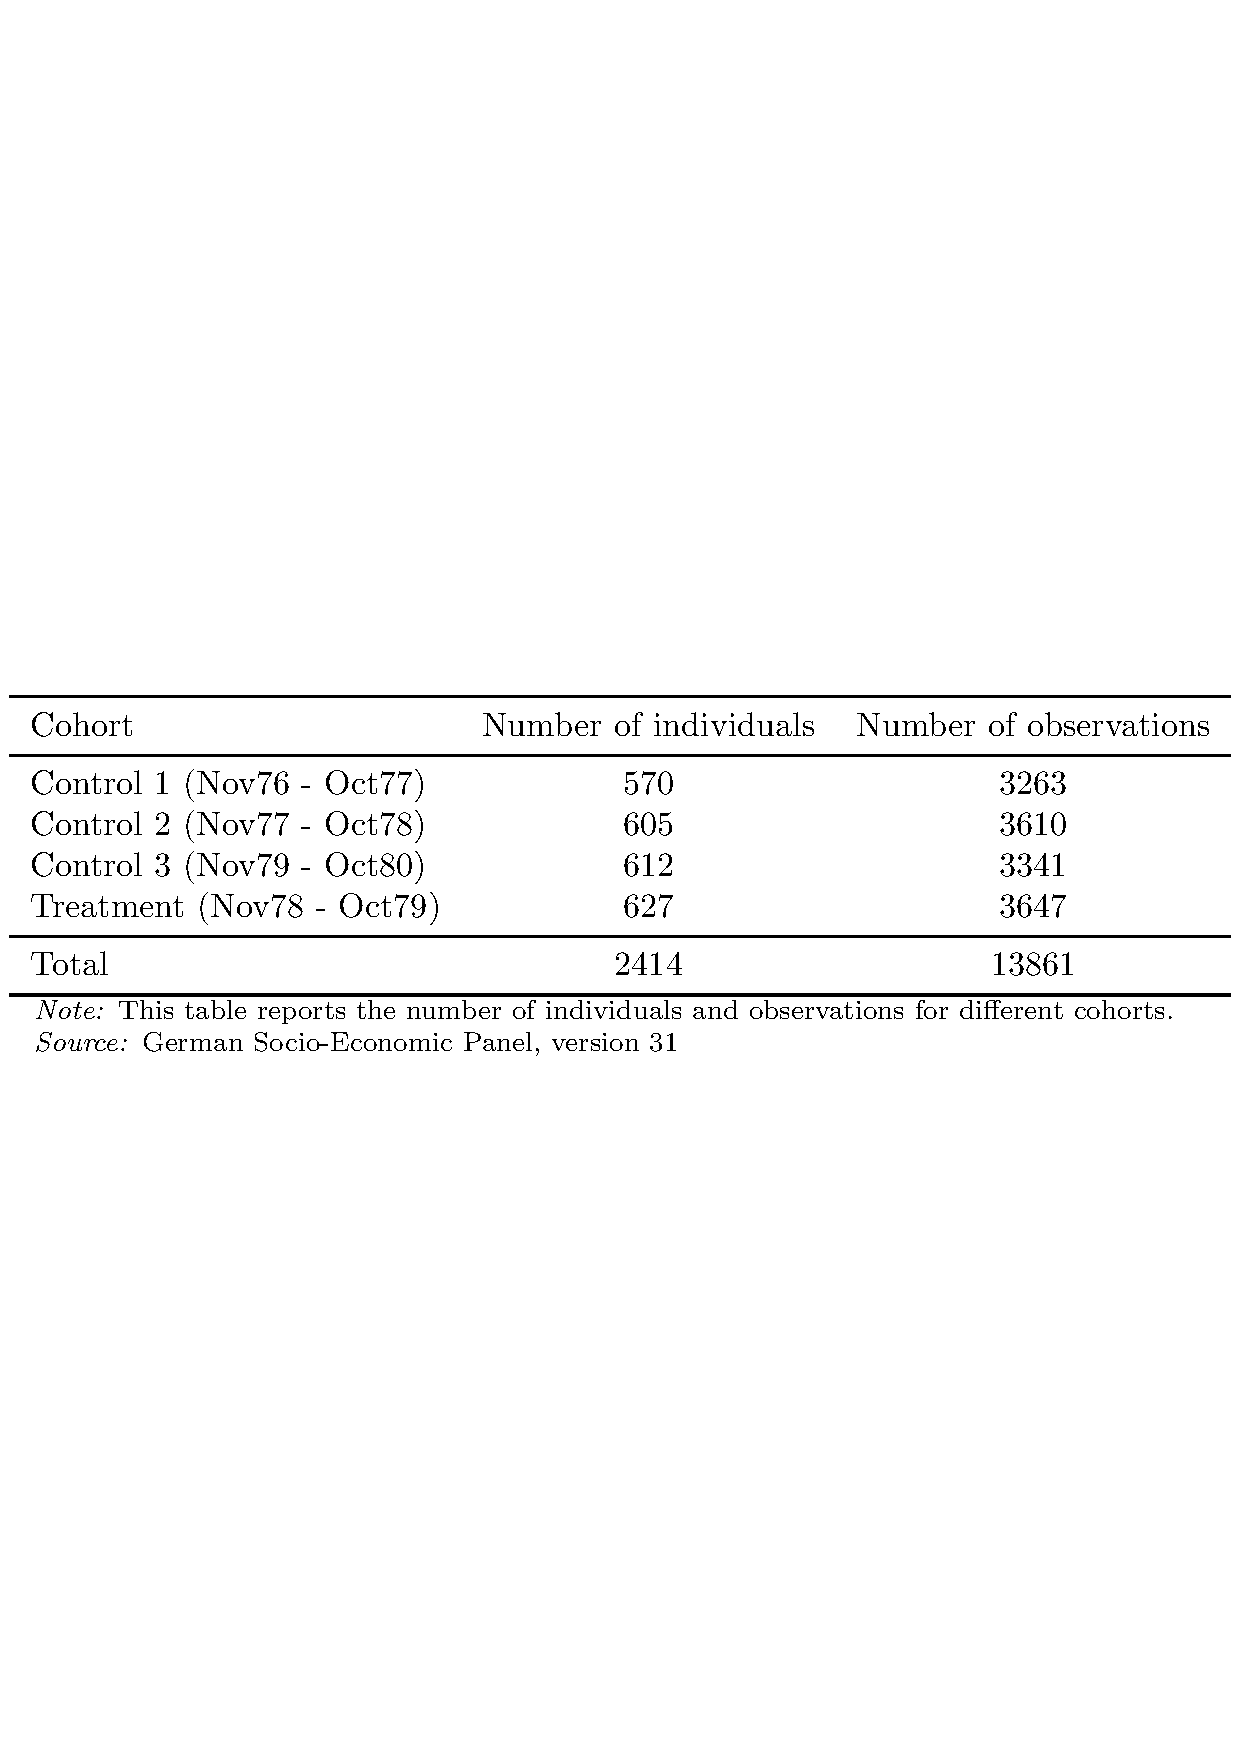
\includegraphics[width=0.8\textwidth]{presentation/data}
%%\caption{Number of observations, per cohort}
%%\end{table}
%\end{frame}
%%------------------------------------------------------
%
%%PARENTAL COVARIATE BALANCE
%\begin{frame}{Pre-determined covariate balance}
%\hyperlink{BACK_XBalance}{\beamerbutton{Back to Parental Covariate Balance}}
%\begin{figure}\label{COVARIATEBALANCEFULL}
%
%
%\begin{tikzpicture}
%	\node[anchor=south west,inner sep=0] at (0,0) {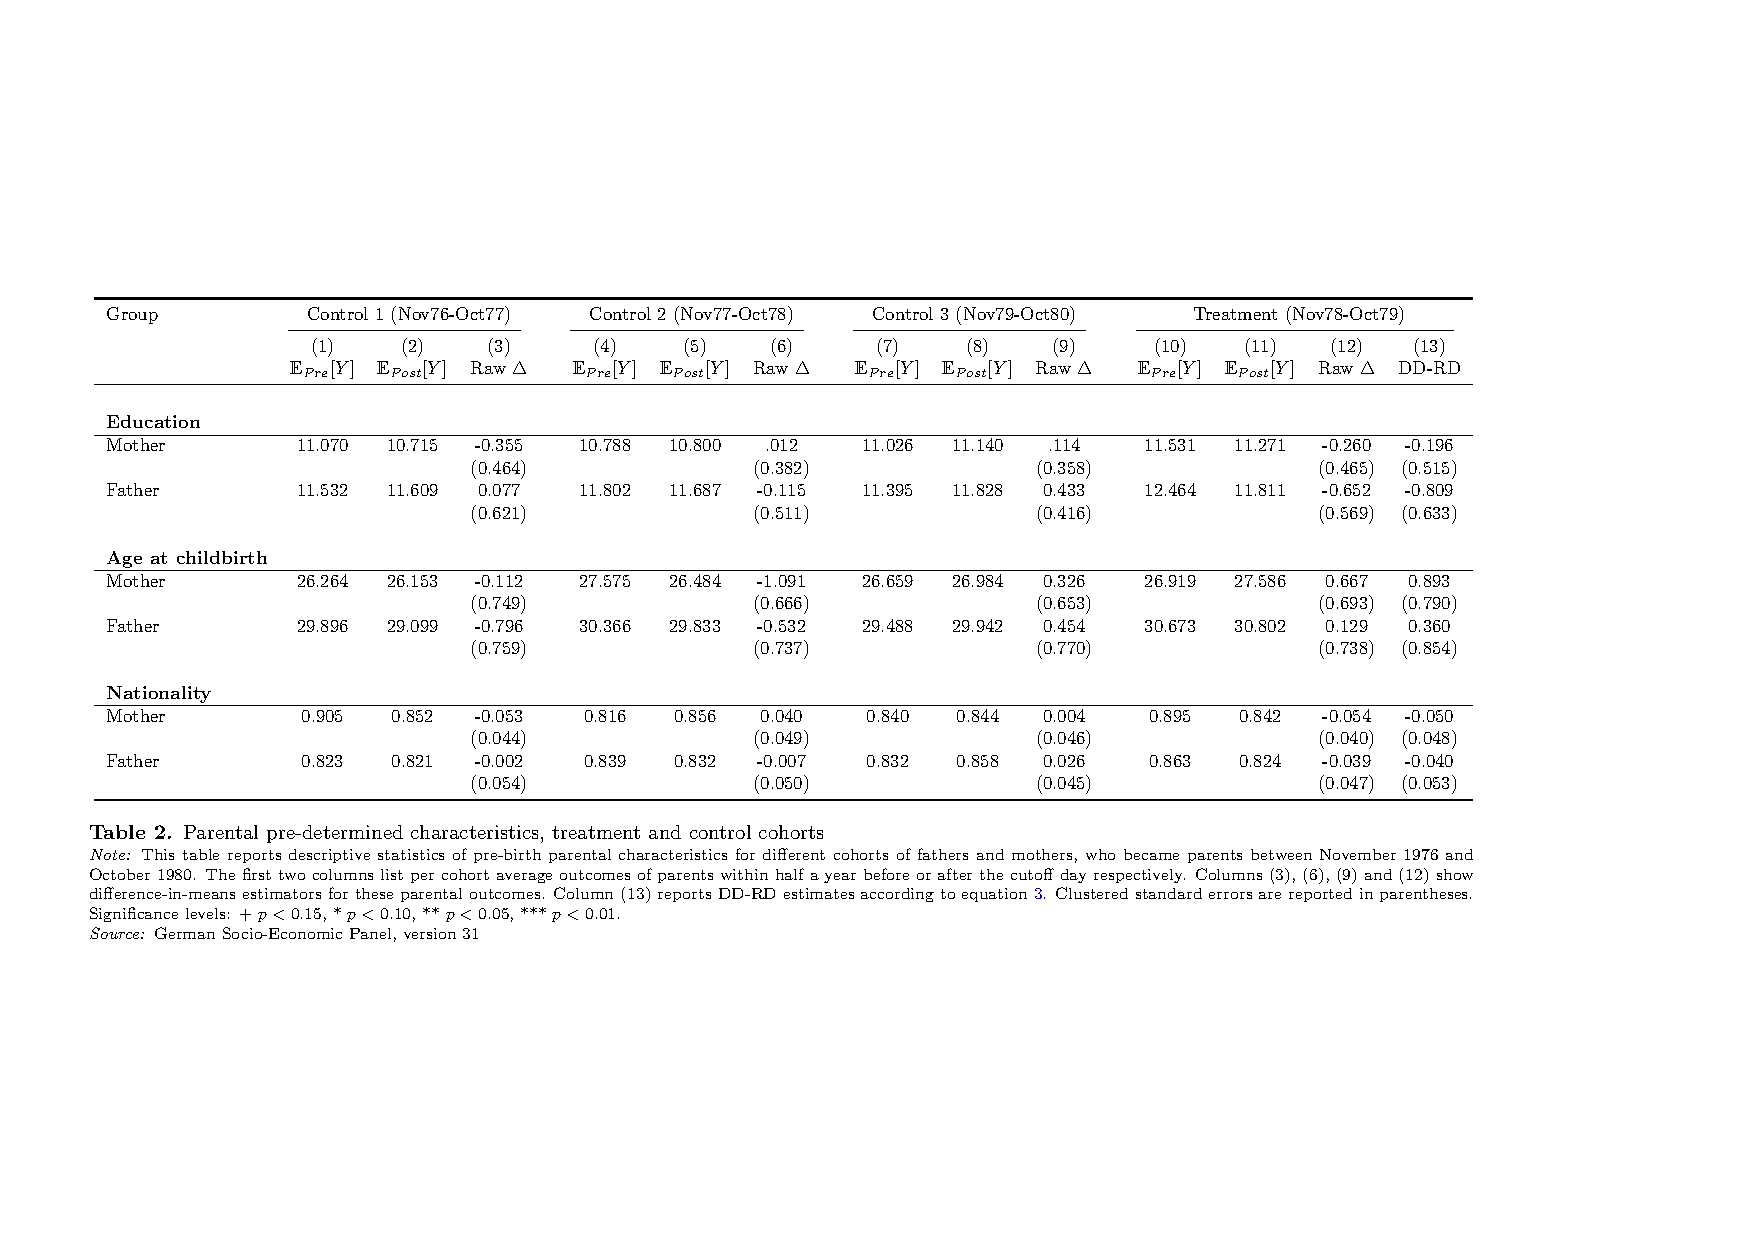
\includegraphics[width=\textwidth]{presentation/parents}};
%	\draw[red,ultra thick,rounded corners] (7.5,1) rectangle (10.5,5);
%	\end{tikzpicture}
%\end{figure}
%\end{frame}
%
%
%
%%------------------------------------------------------
%\begin{frame}
%\begin{figure}\label{HEALTHBEHAVIOR}
%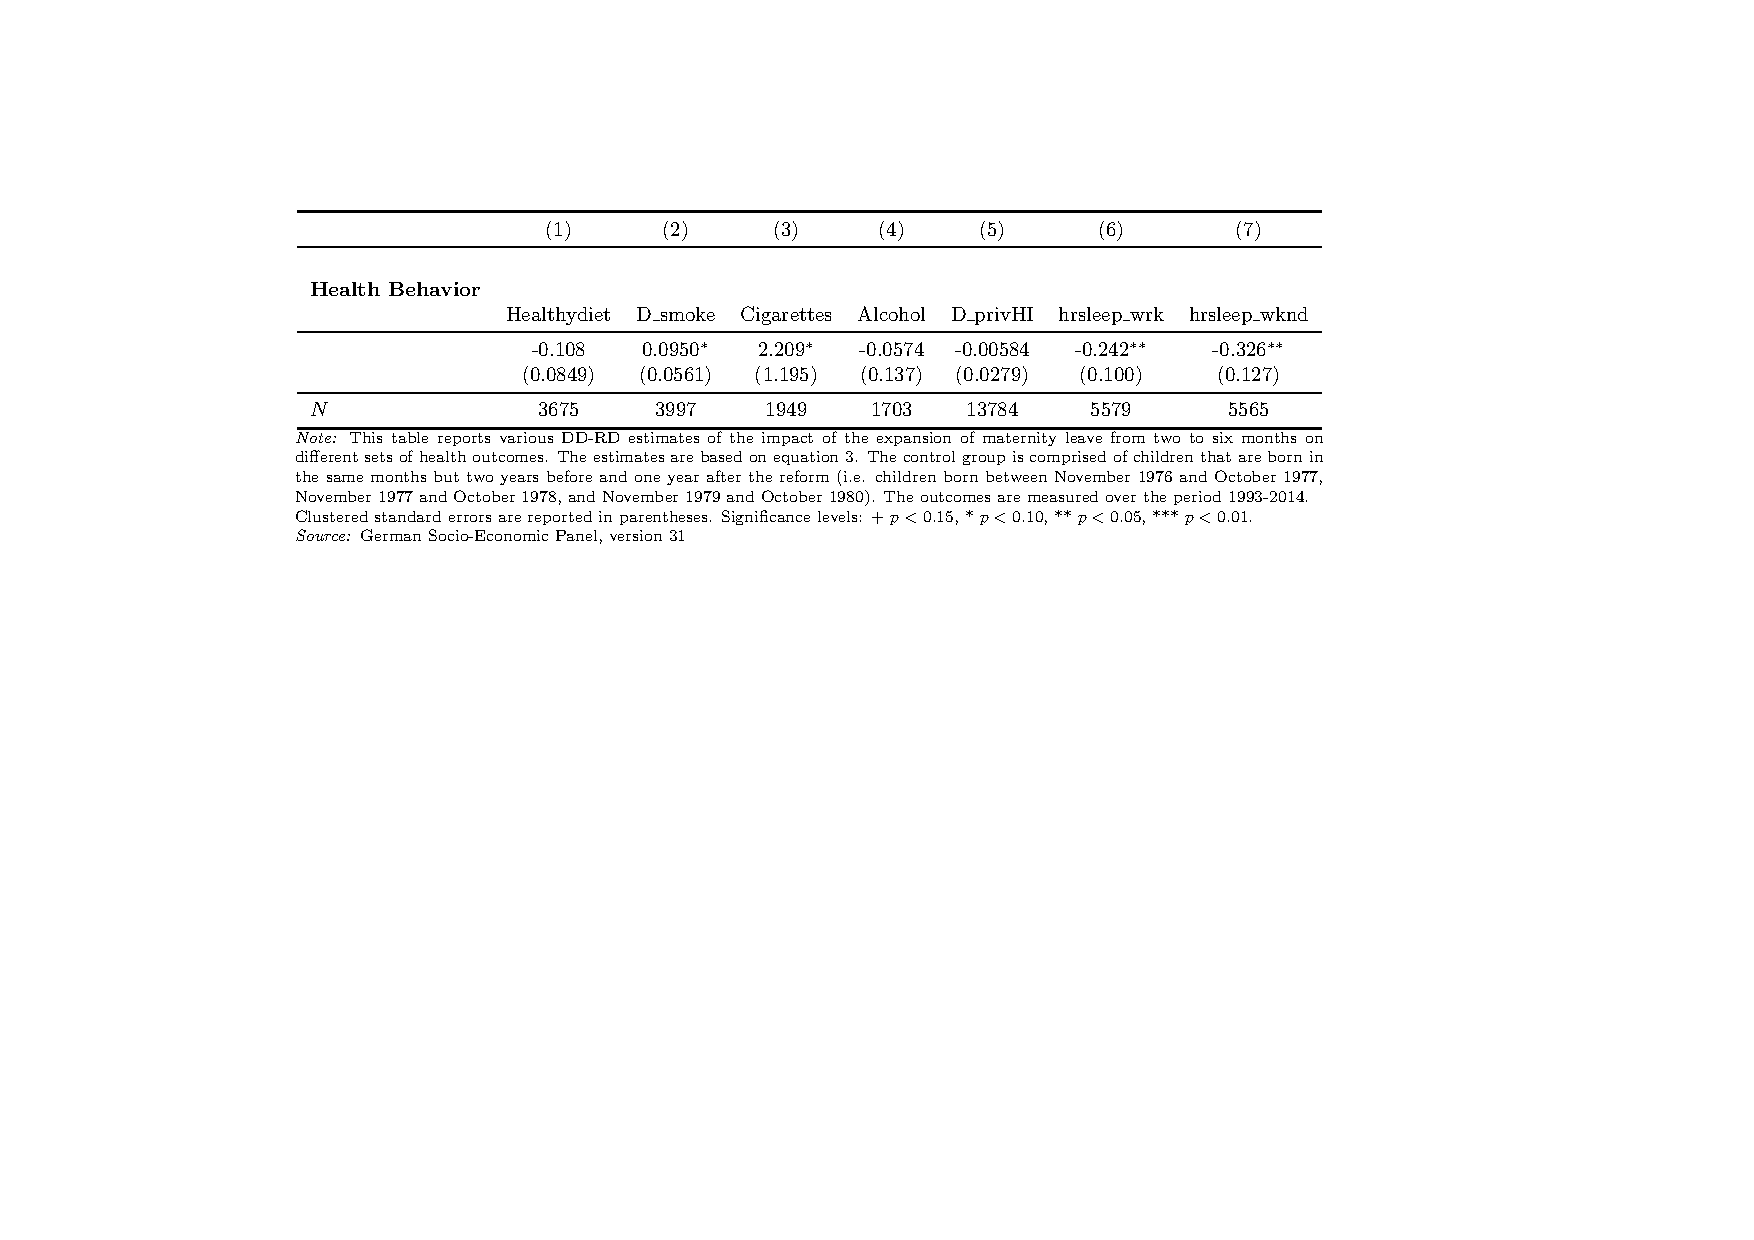
\includegraphics[width=\textwidth]{presentation/HealthBehavior}
%\end{figure}
%\hyperlink{BackMainResults}{\beamerbutton{Back to main results}}
%\end{frame}
%
%
%%------------------------------------------------------
%%MECHANISMS
%\begin{frame}{Mechanisms}
%\hyperlink{BACK_HETERO}{\beamerbutton{Back to Heterogeneity Analysis}}
%\begin{figure}\label{MECHANISMS}
%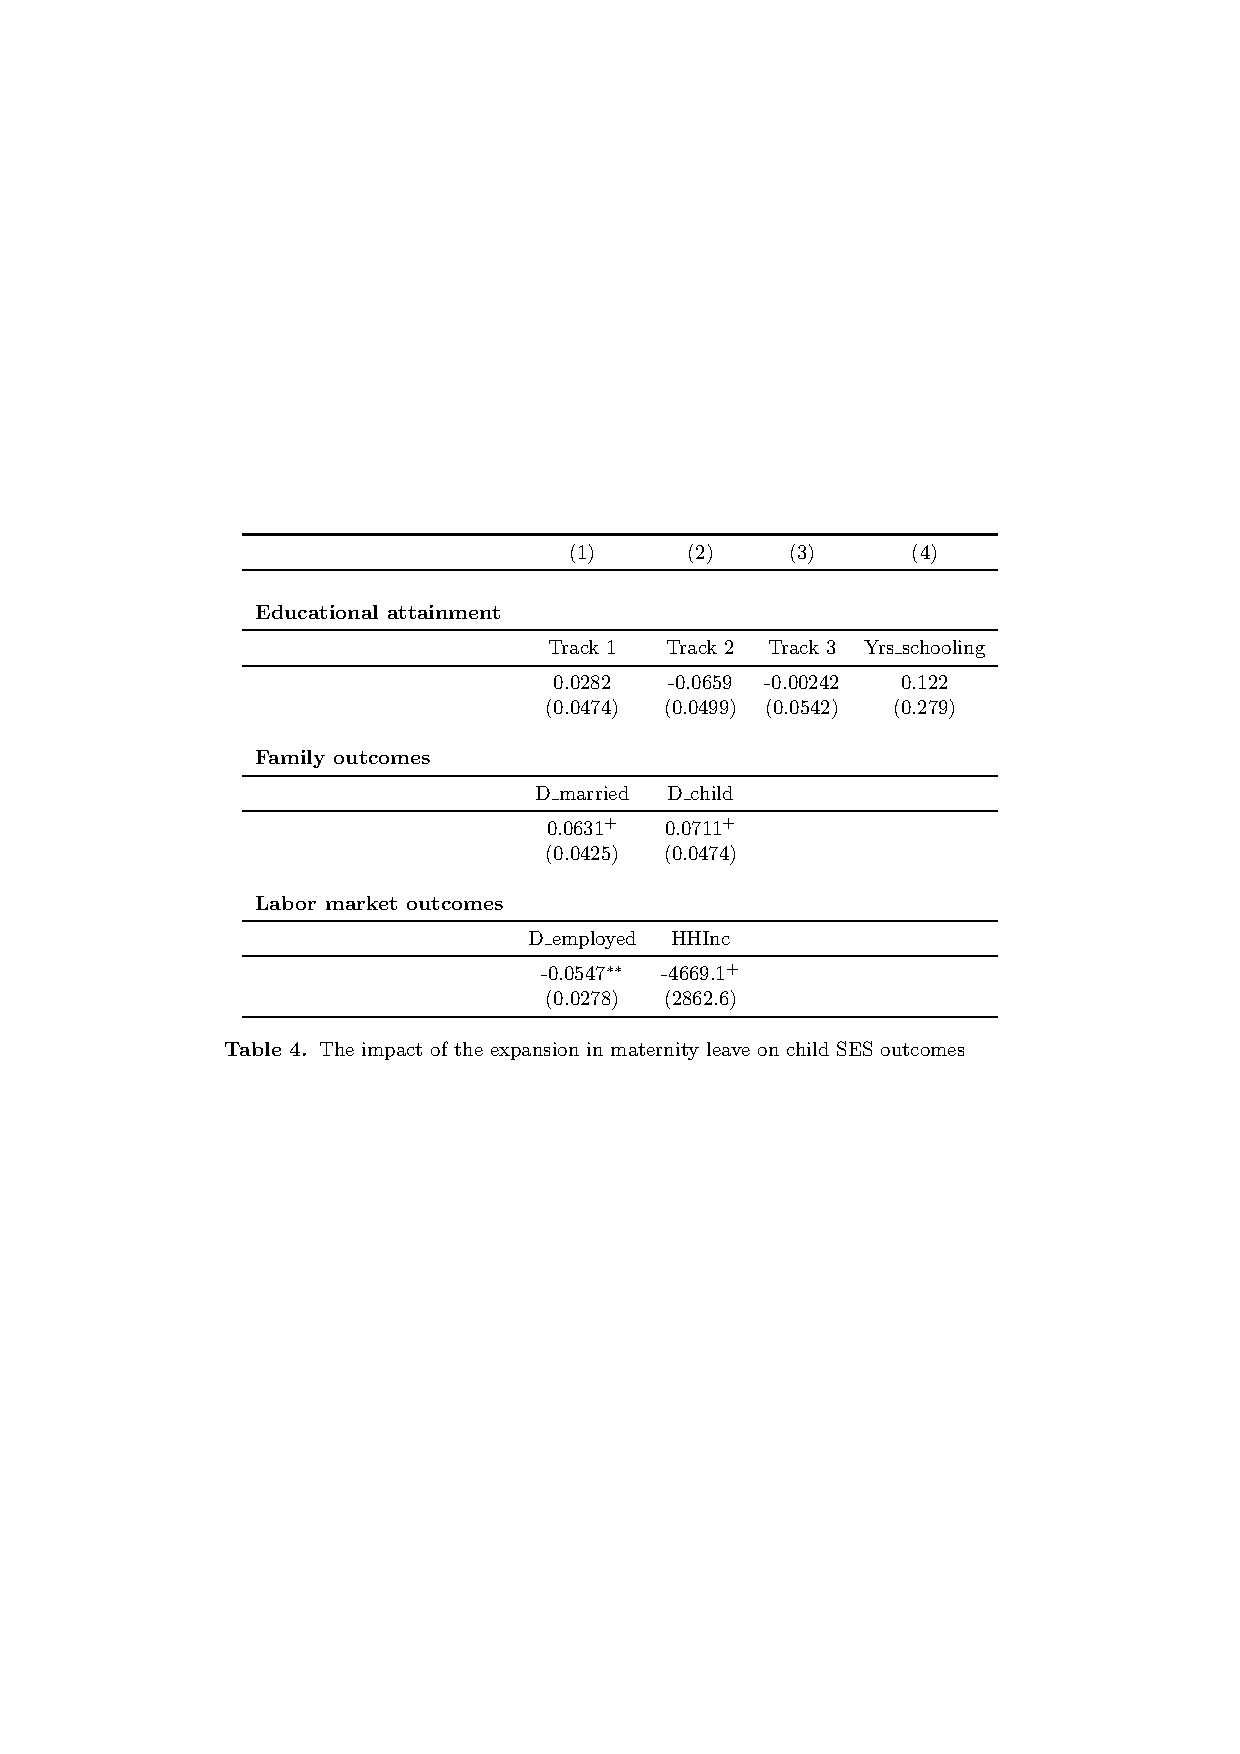
\includegraphics[width=0.75\textwidth]{presentation/Mechanisms_2}
%\end{figure}
%\begin{itemize}
%\item $\Rightarrow$ \mynum{1} and \mynum{3} are verified by D\&S (2012)
%\item \mynum{1} excluded, \mynum{3} possible explanation, \mynum{2} ambiguous effect
%\item Merely suggestive evidence
%\end{itemize}
%\end{frame}

%%%%%%%%%%%%%%%%%%%%%
% MIKROZENSUS
%%%%%%%%%%%%%%%%%%%%%

%------------------------------------------------------
\subsection*{Results Micro Census}
\label{MZ}

\begin{frame}{Further results}

\begin{block}{German Micro Census:}
\begin{itemize}
\item Males less likely to be on sick leave
\item No effects on labor market- and family outcomes; small effect on educational attainment
\end{itemize}
\end{block}
\hyperlink{CONCLUSION}{\beamerbutton{$\triangleright$ Back to conclusion}}
\end{frame}
%------------------------------------------------------
\begin{frame}{\mbox{ Results from the German Micro Census}}
\begin{figure} \begin{center}
\textbf{Health outcomes}
\end{center} 
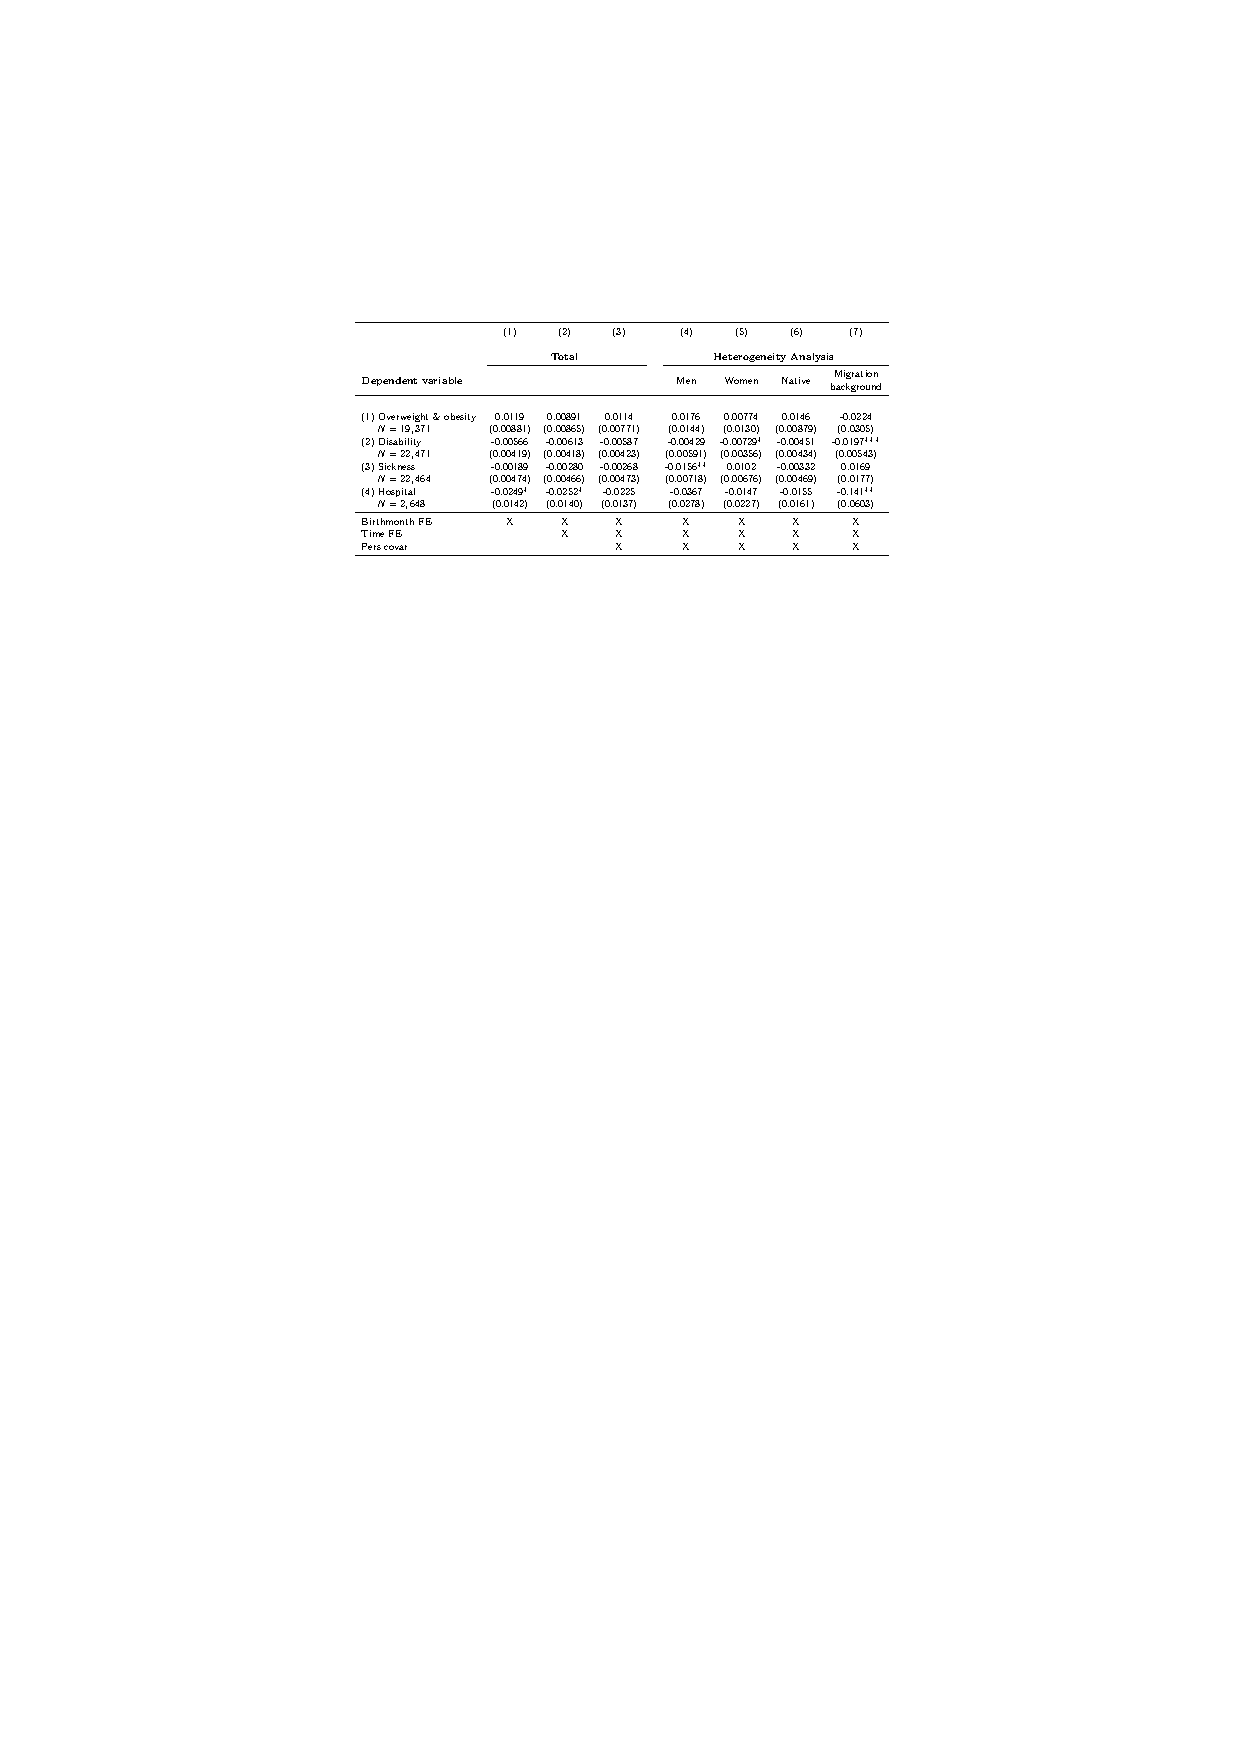
\includegraphics[width = 0.99\linewidth]{../../analysis/graphs/presentation/outcome_MZ_health.pdf}
\end{figure}\vspace{-2.5em}
\tiny \flushleft Note: This table reports various DD-RD estimates of the impact of the expansion of maternity leave from two to six months on different sets of health outcomes. The estimates are based on equation 1. The control group is comprised of children that are born in the same months but one year prior the reform (i.e. children born between  November 1977 and October 1978). Clustered standard errors are reported in parentheses. Significance levels: * \(p<0.10\), ** \(p<0.05\), *** \(p<0.01\).\newline Source: German Micro Census, waves 2005, 2009 and 2013). 
\hyperlink{CONCLUSION}{\beamerbutton{Back to conclusion}}
\end{frame}
%------------------------------------------------------
%SES OUTCOMES
\begin{frame}{Causal effects on socio-economic outcomes}
\begin{figure}
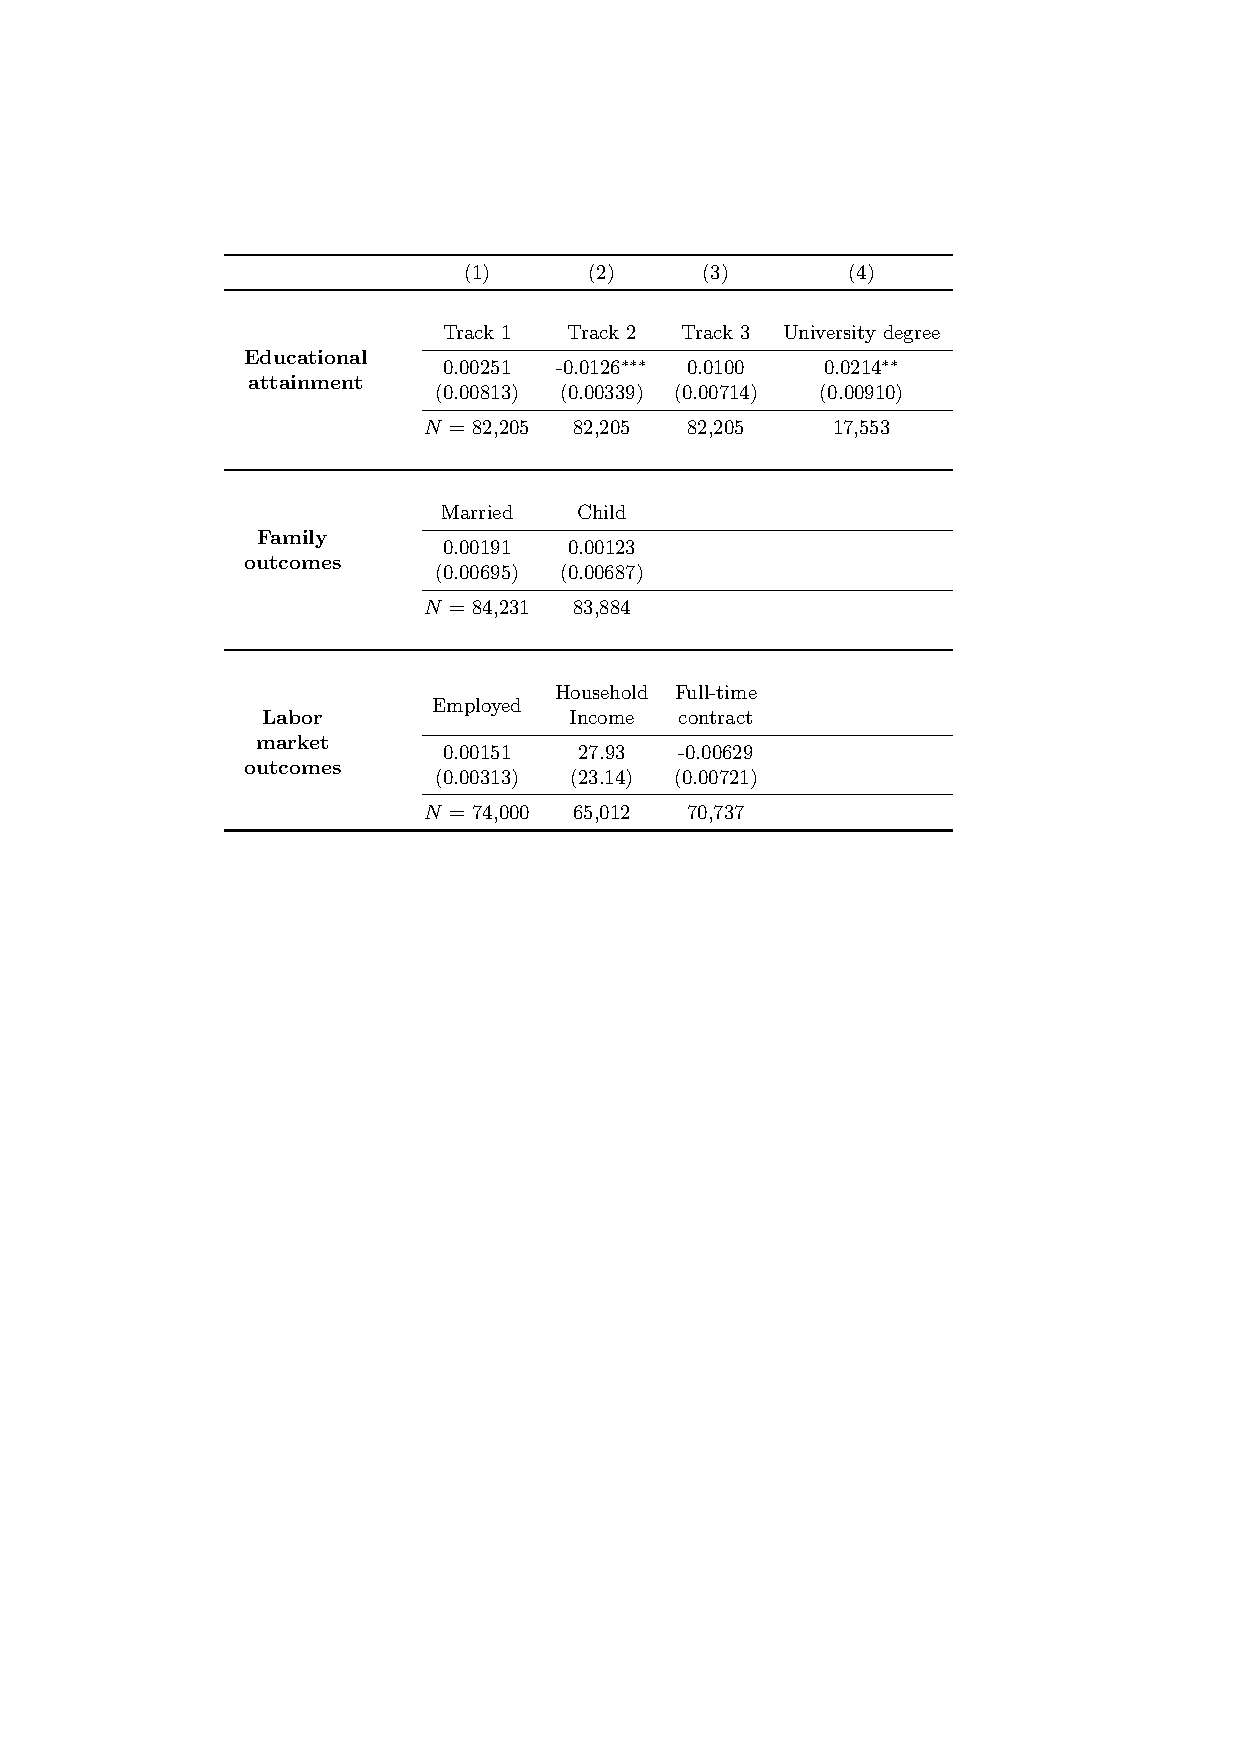
\includegraphics[width=0.6\linewidth]{../../analysis/graphs/presentation/ses_outcomes}
\end{figure}
\vspace{-1.35em}
\tiny \flushleft Note: This table reports various DD-RD estimates of the impact of the expansion of maternity leave from two to six months on different sets of socio-economic outcomes.  Clustered standard errors are reported in parentheses. Significance levels: * \(p<0.10\), ** \(p<0.05\), *** \(p<0.01\). Source: German Micro Census, waves 2005-2013). 
\hyperlink{CONCLUSION}{\beamerbutton{Back to conclusion}}

\end{frame}

	


\end{document}
